\documentclass[onecolumn, groupedaddress, 10pt]{revtex4-1}
\usepackage[utf8]{inputenc}
\usepackage{amsmath}
%\usepackage{mathtools}											% For putting boxes around equations "\Aboxed{}"
\usepackage{amsfonts}
\usepackage{amssymb}
\usepackage{graphicx}											% Use pdf, png, jpg, or eps§ with pdflatex; use eps in DVI
\usepackage[left=2cm, right=2cm, top=2cm, bottom=2cm]{geometry}
\usepackage{dsfont}												% For using C,R,Q,I,N symbols for Rings.
\usepackage{float}												% for controlling the position of objects ie. tables
%\usepackage{breqn}												% For splitting equations using \left and \right across lines
%\usepackage{color}												% For adding color to equations ex.: "/color{red}"
\usepackage[small, bf]{caption}									%Adjust caption size of figures, tables, pictures...
\setlength{\captionmargin}{15pt}
										
\graphicspath{{images/}
              {earthMotionModulationFigure/}
              {images/trial1Results/}}									% folder where images are stored in current directory


% --------------------------- Code for placing two figure side by side ------------------------------------------------------------------
\usepackage{caption}
\usepackage{subcaption}

% --------------------------- Code for the bibliography ---------------------------------------------------------------------------------
\usepackage{natbib}												% For fancy in-text citations
\bibliographystyle{plain}



\begin{document}

\author{Curtis Rau$^{1,2}$}
\author{Colin Gordon$^{1,2}$}
\author{David Witalka$^{1,2}$}
\author{Samuel Akwei-Sekyere$^{1,3}$}
\affiliation{Department of Mathematics$^{1}$ \newline Department of Physics and Astronomy$^{2}$ \newline Neuroscience Program$^{3}$ \newline Michigan State University \newline}

\title{A Novel Method for Removing the Cyclic Frequency Shift due to the Earth's Motion about the Sun from Astronomical Continuous-Wave Data}


\begin{abstract}
In this paper we will introduce the Gustafson Algorithm for removing frequency/phase modulation from a signal.  It takes as input time series data and outputs the original single tone carrier frequency. This method is powerful because it works in the frequency rather than time domain which more easily allows for filtering of the signal and the desired carrier frequency is close to constant over time. Here we will focus on the Gustafson Algorithm's applications to LIGO and the search for gravity waves, but there are many other possible applications for the algorithm such as radio wave astronomy and communications systems using frequency-modulated signals.

\citep{Saulson}
\citep{LSCall}
\citep{Deanna}
\citep{folland}
\citep{griffiths}
\end{abstract}

\maketitle

% --------------------------- Code for the Cover Page ---------------------------------------------------------------------------------

\pagebreak

\section*{Division of Labor}
\textbf{Curtis Rau}
Curtis was the most familiar with the topic and therefore performed the role of group leader identifying topics and problems of interest to be researched. He was alos in charge of writing the algorithm section and the following discussion of the results. The c++ implementation of the algorithm was also done by him. He presented his part in the class presentation.
\begin{itemize}
\item organized topics and problems of interest, directed group research
\item wrote algorithm and discussion of results
\item made figures for presentation and paper
\item wrote rough draft and template for paper
\item Wrote the C++ implementation
\end{itemize}


\textbf{Colin Gordon}
Colin contributed greatly in his research and solving of the phase moulation problem for astronomical signals cause by rotation of the earth using circular orbit approximation. He wrote the introduction to the paper, advised Sam on his section for noise and error analysis, and helped review and edit the paper as a whole. He presented his work in class.
\begin{itemize}
\item researched and solved phase modulation of astronomical signal caused by rotation of earth using circular orbit approximation
\item wrote parts of the introduction
\item reviewed paper and edited
\end{itemize}

\textbf{David Witalka}
David researched and wrote the sections concerning the Nyquist frequency and Carson's rule. He also added the section pertaining to the speed of the Gustafson Algorithm. David edited and reworded the introduction and helped review and edit the paper as a whole. He also created and organized the slides presented in class.
\begin{itemize}
\item created and organized presentation slides
\item researched and edited sections on sampling theorem, Nyquist Frequency and aliasing, Carson’s rule
\item reviewed paper and edited
\end{itemize}

\textbf{Samuel Akwei-Sekyere}
Same researched and wrote the large section on noise and error analysis. He helped greatly in rewording problem sections through out the paper, and greatly expanded the discussion of all topics. Sam placed a major role in reviewing and editing other's sections. He presented his work in class.
\begin{itemize}
\item reviewed and expanded paper (all sections)
\item researched and wrote sections on error analysis, wrote parts of the introduction
\end{itemize}

\pagebreak


\section{Introduction}
General Relativity postulates that information about the spatial distribution of matter in the universe is transmitted via a gravitational field.  Information regarding changes in mass distribution of the universe propagate out through space-time away from the location of that change at the speed of light.  Special events, where the quadrupole moment of the mass distribution changes, emit gravitational radiation.  Extremely violent events in the universe can release enough gravitational radiation to be detectable from Earth.

Recently, the Laser Interferometer Gravitational-Wave Observatory (LIGO) obtained the first emperical evidence of gravitational waves. The discovered ripples in space-time by LIGO was a function of the inspiral of two black holes that eventually merged --- an event that consumed approximately 3 solar masses \citep{abbott}.  It is believed that gravitational wave sources are common in the universe and sources of continuous monochromatic (single frequency) gravitational radiation are predicted to exist --- at least sources with frequencies that persist over many periods \cite{}. Neutron stars have also been implicated as one of the prime sources of gravitational waves.  These stars are expected to emit single frequency waves over long periods of time.  Additionally, it has also been proposed that an appreciable fraction of detectable gravitational waves emmitters are binary neutron star systems --- two neutron starts orbiting around each other.

A fundamental challenge to efficient detection of gravitational waves is that orbiting binary neutron star systems invoke frequency modulations which reduce the power of the carrier frequency and distributes it to higher and lower harmonics.  In essence, the power of the signal is dispersed over a range of side-band frequencies; this phenomenon is due to the Doppler effect arising from the Earth's motion relative to the source of the wave. Since the noise observed in the LIGO data is approximately Gaussian and of low signal-to-noise ratio, the extraction of reliable information about gravitational waves is arduous.

In order to calculate the carrier frequency of the wave, consider the wave as one emitted from a source that is megaparsecs away (potentially in other galaxies). By virtue of its distance, the spherical coordinates will not change significantly and the source will move relative to the sun with nearly constant velocity over the time we collect data. By the same token, the sun will experience the monochromatic wave produced by the source as truly monochromatic, while its detection on the Earth will be in the form of a frequency modulated signal.

\begin{figure*}[ht]
	\centering
	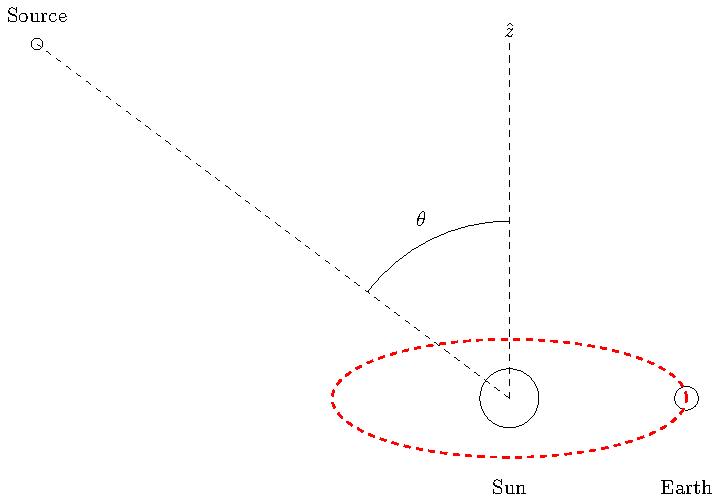
\includegraphics[width=.75\linewidth]{earthMotionModulationFigure.pdf}
	\caption{\label{fig:earthMotionModulationFigure}}
\end{figure*}

By assuming that the wave travels at the speed of light, we can capture it as a Lorentz invariant 4-vector with the carrier frequency being the first entry and the second through fourth entries is the wave number. In order to transform it in the Earth's frame we apply an instantaneous Lorentz boost on the 4-vector; the instantaneous boost takes the direction of the motion of the Earth and the velocity of the the Earth in orbit into consideration. Without loss of generality, the Earth's orbit is captured in the $xy$ plane. The 4-vector is written in the perspective that assumes the wave is a plane wave which travels towards the Sun on a trajectory that is on the $xz$ plane. The matrix with the trigonometric functions projects that 4-vector on a new basis and effectively forcing the second component of the 4-vector to be in the direction of motion of Earth. The matrix with the Betas and gammas is a Lorentz transformation that applies on 1st and 2nd component. now the 4-vector is in the frame of the Earth. After all of this, we could apply rotations or whatever to change the spatial coordinate system but we only care about the frequency which is invariant under any of those changes.

\begin{align}
\label{eqn: new k}
\mathbf{K} &=
\left( \begin{array}{cccc}
	    \gamma   & -\gamma \beta & 0 & 0 \\
	-\gamma \beta &    \gamma    & 0 & 0 \\
	      0      &       0      & 1 & 0 \\
	      0      &       0      & 0 & 1
\end{array} \right)
\left( \begin{array}{cccc}
	1 &               0             &              0               & 0 \\
	0 & -\sin (\omega_e t + \phi_e) &  \cos (\omega_e t + \phi_e)  & 0 \\
	0 & -\cos (\omega_e t + \phi_e) &  -\sin (\omega_e t + \phi_e) & 0 \\
	0 &               0             &              0               & 1
\end{array} \right)							 
\left( \begin{array}{c}	
	   \omega_0 / c   \\
	- k \sin \theta \\
	        0       \\
	- k \cos \theta    
\end{array} \right)																			\\
&=
\left( \begin{array}{c}
	\gamma \left(\omega_0 / c - \beta k \sin \theta \sin (\omega_e t + \phi_e)\right) \\
	\gamma \left(-\beta \omega_0 / c + k \sin \theta \sin (\omega_e t + \phi_e)\right) \\
	           \gamma k \sin \theta \cos (\omega_e t + \phi_e)           \\
	                           - k \cos \theta
\end{array} \right)   ,
\end{align}

where $\theta$ is the polar angle from the axis perpendicular to the orbit of Earth, $\gamma$ is the Lorentz factor from special relativity, $\omega_e$ is the angular frequency of the Earth's rotation about the Sun, $c$ is the speed of light and $\beta$ is the velocity of Earth's orbit divided by the speed of light.

From this formulation we can infer that the new instantaneous frequency in the Earth's frame can be given by:

\begin{equation}
\omega (t) = \omega_0 \gamma \left( 1 - \beta \sin \theta \sin (\omega_e t + \phi_e) \right). 
\end{equation}

Since the phase refers to the time integral of the frequency, the expression for the wave being sought after is the real part of the following: 

\begin{align}
h(t)    &= h_0 e^{i \left( \omega' t + \Gamma \cos (\omega_e t + \phi_e) \right)}		\\
\omega' &= \gamma \omega_0															\\
\Gamma  &= \frac{\gamma \beta \omega_0 \sin \theta}{\omega_e}
\end{align}


where $h_0$ is the amplitude of the wave, $\Gamma$ is the modulation index, $\omega_0$ is the frequency of the wave to be detected, $\phi_0$ is the phase of the wave to be detected at $t=0$, $\phi_e$ is the relative phase difference between the Earth's rotation about the Sun and the wave to be detected.

An important note is that $\Gamma$ is a function of only the azimuthal angle of the source with respect to the normal of the gallactic plane. This algorithm will also work perfectly well with any frequency modulated wave produced similar to the above. One likely case scenario is when the compact stars are in a binary system so one or both objects produce waves but the stars rotate around each other causing an analogues phase modulation.  In this way there could be applications for the Gustafson algorithm in areas outside of gravitational waves in areas such as radio wave astronomy and communications using frequency modulated signals. We attempt to keep the discussion of the algorithm and the results as general as possible for this reason.

\section{The Gustafson Algorithm}
The goal of this paper is to propose a search algorithm that can efficiently detect the presence of frequency modulated waves, while being robust against noise.  A brute force way to accomplish this is to take the inner product of 

\begin{equation}
h(t) = h_0 e^{i\left( \omega_0 t + \phi_0 + \Gamma \cos (\omega_1 t + \phi_1 ) \right)}
\end{equation}

with the data for different values of $\omega_0$, $\omega_1$, $\phi_0$, $\phi_1$, and $\Gamma$.  This is effectively a Fourier Transform as a function of the the 4 search parameters

\begin{align}
\hat{f}(\omega_0, \omega_1, \phi_1, \Gamma) = \int f(t) e^{-i\left( \omega_0 t + \phi_0 + \Gamma \cos (\omega_1 t + \phi_1 ) \right)} dt
\end{align}

We would expect this to produce a something like a delta function, or at least a Dirchlet Kernel because of discretization.  The ammount of time it will take to perform this computation is $\mathcal{O} (N_tN_{\omega_0}N_{\omega_1}N_{\phi_1}N_\Gamma)$, where $N_t$ denotes the number of data points, and the other $N_x$ is the number of steps in $x$ that the search will take.  Typically for a Discrete Fourier Transform (DFT) the number of steps in frequency is equal to the number of data points: $N_t=N_{\omega_0}=N_{\omega_1}$ \cite{}.  Physically this means the frequency resolution of the DFT is proportional to the duration of the time series over which the DFT is taken.  Thus the computation time for the brute force method goes as $\mathcal{O} (N_t^3N_{\phi_1}N_\Gamma)$.  

Of particular interest is the case when the signal is buarried deep within non-coherent noise.  A conventional way to improve the signal to noise ratio (SNR) is to simply take more data.  This assumes the signal is more periodic than noise.  (why does this yeald a better snr??????)  The problem with taking more data however is that the brute force method computational time is proportional to $N_t^3$.  We will now introduce the Gustafson Algorithm which is roughly a factor of $N_t$ faster than the brute force method.

To derive the Gustafson Algorithm we start by assuming the data $f(t)$ takes on the form of a complex frequency modulated wave.  The actual data will be real, but this complecation makes the derivation almost impossible.  Later it will be shown that starting with the complex wave is perfectly valid.  We demodulate the wave and take the Fourier Transform of both sides.

\begin{align}
h_0 e^{i\left( \omega_0 t + \phi_0 + \Gamma \cos (\omega_1 t + \phi_1 ) \right)} &= f(t) 												\\
h_0 e^{i\phi_0} e^{i\omega_0 t} &= f(t) e^{-i\Gamma \cos (\omega_1 t + \phi_1)}															\\
h_0 e^{i\phi_0} \mathcal{F}_t \left[ e^{i\omega_0 t} \right] &= \mathcal{F}_t \left[ f(t) e^{-i\Gamma \cos (\omega_1 t + \phi_1)} \right]
\end{align}

Define $F_t[f(t)](\omega) = \hat{f}(\omega)$, and invoking the convolution theorem

\begin{equation}
\label{eqn:derivation:convolutionThmStep}
\frac{h_0 e^{i\phi_0}}{\sqrt{2\pi}} \delta (\omega_c - \omega) = \hat{f}(\omega) \star F_t \left[ e^{-i\Gamma \cos (\Omega t + \phi)} \right]
\end{equation}

The Jacobi-Anger Expansion, which comes up often in this paper, has the form \cite{}:

\begin{equation}
\label{eqn:jacobiAnger}
e^{iz\cos (\theta)} = \sum_{n=-\infty}^{\infty} e^{in\pi/2} J_n(z) e^{in\theta}
\end{equation}

so equation \ref{eqn:derivation:convolutionThmStep} becomes

\begin{align}
\label{eqn:derivation:jacobiAngerInsertion}
\frac{h_0 e^{i\phi_0}}{\sqrt{2\pi}} \delta (\omega - \omega_0)
&=
\hat{f}(\omega)
\star \mathcal{F}_t \left[ \sum_{n=-\infty}^{\infty} e^{in\pi/2} J_n(-\Gamma) e^{in(\omega_1 t + \phi_1)} \right]
\end{align}

Even order Bessel Functions are even, and odd order Bessel Functions are odd \cite{}.  Explicitly

\begin{align}
	J_n(-z) &= (-1)^n J_n(z)
\end{align}

Using this fact

\begin{align}
\mathcal{F}_t \left[ \sum_{n=-\infty}^{\infty} e^{in\pi/2} J_n(-\Gamma) e^{in(\omega_1 t + \phi_1)} \right]
&= \sum_{n=-\infty}^{\infty} (-1)^n e^{in\pi/2} e^{in\phi_1} J_n(\Gamma) \mathcal{F}_t \left[e^{in\omega_1 t} \right]	 \\
&= \frac{1}{\sqrt{2\pi}}\sum_{n=-\infty}^{\infty} e^{in(\phi_1 - \pi/2)} J_n(\Gamma) \delta (\omega - n\omega_1)
\end{align}

In the previous step we used the linearity of the Fourier Transform $F_t[c \cdot f(t)] = c \cdot F_t[f]$.  Equation \ref{eqn:derivation:jacobiAngerInsertion} becomes

\begin{align}
h_0 e^{i\phi_0} \delta (\omega - \omega_0) = \hat{f}(\omega)
\star
\left[ \sum_{n=-\infty}^{\infty} e^{in(\phi_1 - \pi/2)} J_n(\Gamma) \delta (\omega - n\omega_1) \right]
\end{align}

Performing the convolution 

\begin{align}
\hat{f}(\omega) \star \delta (\omega - n\omega_1) 
&= \int \hat{f}(\omega - \widetilde{\omega}) \delta(\widetilde{\omega} - n\omega_1) d\widetilde{\omega}			\\
&= \hat{f} (\omega - n\omega_1)
\end{align}

brings us to the almost final answer:

\begin{align}
h_0 e^{i\phi_0} \delta (\omega - \omega_0) = \sum_{n=-\infty}^{\infty} e^{in(\phi_1-\pi/2)} J_n(\Gamma) \hat{f} (\omega - n\omega_1)
\end{align}

For clarity and later convenience let's have $n\to -n$.  We will use the other property of the Bessel Functions: \cite{}

\begin{align}
J_{-n} (z) &= (-1)^n J_n(z)
\end{align}

Which brings us to the Gustafson Algorithm:

\begin{align}
\label{eqn:gustafsonAlgorithm}
\boxed{h_0 e^{i\phi_0} \delta (\omega - \omega_0) = 2 \sum_{n=-\infty}^{\infty} e^{-in(\phi_1+\pi/2)} J_n(\Gamma) \hat{f} (\omega + n\omega_1)}
\end{align}


An erroneous factor of two has been added to the algorithm which, as we will see, makes it suitable for use with real data.  It is not obvious weather or not this algorithm in its current form can be used on real data because it assumed a complex waveform.  This assumption allowed for a clean demodulation, which is spoiled if one takes the real of this function.  This is due to the nonlinearity of the real opperator as demonstrated by

\begin{align}
\Re \{ a \cdot b \} \neq \Re \{ a \} \cdot \Re \{ b \}; \qquad a,b \in \mathds{C}
\end{align}

We can use equation (\ref{eqn:gustafsonAlgorithm}) as a guess as to find the form that will work with a real valued waveform.  Upon comparison of the Fourier transforms of the complex and real waveforms (see appendices A and B) we see they are very similar.  The real looks like the complex with the addition of terms that are mirrored about $\omega=0$.

What would we have to do to get the fourier transform of the real to look exactly like the fourier transform of the complex wave?  Unsurprisingly not much because they are such similar functions.  All we would have to do is drop the extra mirrored terms.


We would only have to multiply each term by some phase factor to get the real fourier transform to look like the sum of two complex fourier transforms.  After adding in the phase factors we plug the  fourier transform of the real wave into the Gustafson Algorithm which will yeald two delta functions now instead of one (because the fourier transform of the real is the sum of two complex wave fourier transforms).  One delta function will be at $+\omega_0$, this is the one of interest, and the other will be at $-\omega_0$.  (A much more rigerous explanation of this is needed.)  If we carry the search out over only positive values of $\omega_0$ then we can throw out all terms in red of the fourier transform of the real wave because they are inconsequential to the algorithm.  Finally, the phase terms that were added to the foureier transform of the real to make it look like the complex can be encorperated into the Guatafson Algorithm.  The only remaining thing to do is multiply the Gustafson Algorithm by two (explain why).


\subsection{Discussion of The Gustafson Algorithm}
It is not explicitly obvious how The Gustafson Algorithm, Eq. \ref{eqn:gustafsonAlgorithm}, can be used as a search algorithm capable of determining the values $h_0, \omega_0, \omega_1, \phi_0, \phi_1, \Gamma$.  In this section we seek to make obvious what Eq. \ref{eqn:gustafsonAlgorithm} can do.  

Assume the data takes on the real form of a frequency modulated wave.

\begin{align}
\label{eqn:realData}
f(t) = \Re \left\{ h_0 e^{i\left( \omega_0 t + \phi_0 + \Gamma \cos( \omega_1 t + \phi_1 ) \right)} \right\}
\end{align}

Initially we do not know the values of $\omega_0, \omega_1, \phi_0, \phi_1, \Gamma$.  To determin these values we will try the values $\widetilde{\omega}_0, \widetilde{\omega}_1, \widetilde{\phi}_1, \widetilde{\Gamma}$ in the Gustafson Algorithm.

\begin{align}
G_{\widetilde{\omega}_0,\widetilde{\omega}_1,\widetilde{\phi}_1,\widetilde{\Gamma}} \left[ \hat{f}(\omega) \right] 
= \sum_{n=-\infty}^{\infty} e^{-in(\widetilde{\phi}_1+\pi/2)} J_n(\widetilde{\Gamma}) \hat{f} (\omega + n\widetilde{\omega}_1)
\end{align}

To see what this will yeald we substitute the Fourier Transform of the real of the waveform, equation (\ref{eqn:realFourierTransform}), into the above equation

\begin{align}
G_{\omega_0,\omega_1,\phi_1,\Gamma} \left[ \hat{f}(\omega) \right] = 
&\frac{h_0}{2} \sum_{m,n=-\infty}^{\infty} e^{i(m\phi_1-n\widetilde{\phi}_1)} J_n(\widetilde{\Gamma}) J_m (\Gamma)				\nonumber \\
&\times \left[
e^{i(\phi_0 + (m-n)\pi/2)} \delta(\omega - \omega_0 + n\widetilde{\omega}_1 - m\omega_1)
+ e^{-i(\phi_0 + (m+n)\pi/2)} \delta(\omega + \omega_0 + n\widetilde{\omega}_1 - m\omega_1)
\right]
\end{align}






%Where $\delta_{m}$ is the Kronecker Delta.  \cite{}  
%To put this equation in a more suggestive form we introduce the sideband mismatch number $l=m-n$.  This integer gives ???????

%\begin{align}
%&\frac{h_0}{2} \sum_{n,l=-\infty}^{\infty} e^{il\phi_1} e^{in(\phi_1-\widetilde{\phi}_1)} J_n(\widetilde{\Gamma}) J_{n+l} (\Gamma)				\nonumber \\
%&\qquad \qquad
%\times \left[
%e^{i\phi_0} e^{il\pi/2} \delta(\omega - \omega_0 + n(\widetilde{\omega}_1 - \omega_1) - l \omega_1)
%+ e^{-i\phi_0} e^{-il\pi/2} e^{-in\pi} \delta(\omega + \omega_0 + n(\widetilde{\omega}_1 - \omega_1) - l \omega_1)
%\right]
%\end{align}

%-------------------- w != w0 & w1 != w1~ --------------------

This needs to be treated in cases.  

\textbf{Case 1:}  Let's consider the most likely case when $\omega \neq \omega_0$ and $\omega_1 \neq \widetilde{\omega}_1$.  Let's examin the term $\delta(\omega - \omega_0 + n\widetilde{\omega}_1 - m\omega_1)$ in the above equation in detail.  This delta function appears in the double sum and is a function of both $m$ and $n$, so the $n\widetilde{\omega}_1 - m\omega_1$ is changing over the sums whereas the value $\omega - \omega_0$ is constant (not a function of $m$ or $n$).  This delta is non-zero only if

\begin{align}
                0 &= \omega - \omega_0 + n\widetilde{\omega}_1 - m\omega_1		\\
\omega_0 - \omega &= n\widetilde{\omega}_1 - m\omega_1
\end{align}

This can happen twice or never.  By the Euclidean Algorithm, the delta will only be non-zero if

\begin{align}
\gcd \left( \widetilde{\omega}_1, \omega_1 \right) = \omega_0 - \omega
\end{align}

If this is false then the sum is zero.  If it is true then call the values for $m$ and $n$ that make it true $\pm m_o$ and $\mp n_o$.  So then the sum is 


~~~ Placeholder for equation ~~~


%-------------------- w = w0 & w1 != w1~ --------------------
\textbf{Case 2:}  Now consider the case when $\omega = \omega_0$ and $\omega_1 \neq \widetilde{\omega}_1$.  The term $\delta(\omega - \omega_0 + n\widetilde{\omega}_1 - m\omega_1)$ will only be non-zero if

\begin{align}
\widetilde{\omega}_1 = \frac{m}{n} \omega_1
\end{align}

Again this can happen twice or never.  If this is false then the sum is zero.


~~~ Placeholder for equation ~~~


%-------------------- w != w0 & w1 = w1~ --------------------
\textbf{Case 3:}  Now consider the case when $\omega \neq \omega_0$ and $\omega_1 = \widetilde{\omega}_1$.  The term $\delta(\omega - \omega_0 + n\widetilde{\omega}_1 - m\omega_1)$ will only be non-zero if

\begin{align}
\omega - \omega_0 = (n-m)\widetilde{\omega}_1
\end{align}

Again this can happen twice or never.  If this is false then the sum is zero.


\textbf{Cases 1-3:}  In all of these cases

%-------------------- w != w0 & w1 = w1~ --------------------
\textbf{Case 4:}  Now consider the case when $\omega = \omega_0$ and $\omega_1 = \widetilde{\omega}_1$.  The term $\delta(\omega - \omega_0 + n\widetilde{\omega}_1 - m\omega_1)$ will only be non-zero if $m=n$ which will happen an infinite number of times.  The sum becomes

%This treatment does not include the \delta(\omega + \omega_0 + n\widetilde{\omega}_1 - m\omega_1) term of the fourier transform.
\begin{align}
\frac{h_0}{2} e^{i\phi_0} \delta(0) \sum_{n=-\infty}^{\infty} e^{in(\phi_1-\widetilde{\phi}_1)} J_n(\widetilde{\Gamma}) J_n (\Gamma)
\end{align}

\textbf{Case 4a:} Now if we let $\Gamma = \widetilde{\Gamma}$ and $\phi_1 = \widetilde{\phi}_1$ then the sum becomes

\begin{align}
\frac{h_0}{2} e^{i\phi_0} \delta(0) \sum_{n=-\infty}^{\infty} J_n^2 (\Gamma) = \frac{h_0}{2} e^{i\phi_0} \delta(0)
\end{align}

So if we guess every search parameter correctly, $\omega = \omega_0$, $\omega_1 = \widetilde{\omega}_1$, $\Gamma = \widetilde{\Gamma}$, and $\phi_1 = \widetilde{\phi}_1$, then we recover the 

%call $l$ the sideband mismatch number.


%- Bessel functions have the property \cite{}

%\begin{align}
%\sum_{n=-\infty}^{\infty} J_n (x) J_{n+m} (x) = \delta_{m}
%\end{align}

%Where $\delta_{m}$ is the Kronecker Delta.  \cite{}  


\section{Carson's Rule and the Nyquist frequency}
In order too fully reconstruct the carrier frequency we would need to take an infinite sum over the sidebands. As this is impractical and unnecessary as many terms are insignificant, we need to find a way to limit the number of sidebands we are summing over. The first problem is locating the sidebands' characteristic frequency. There are infinite sideband frequencies and eventually they will be higher than the Nyquist frequency which will cause aliasing of the sideband frequency. The Nyquist frequency, $\psi_N$, is defined as the maximum frequency that can be accurately reconstructed and is equal to half of the sampling frequency, $\psi_s$.

\begin{equation}
\psi_N = \frac{1}{2}\psi_s
\end{equation}

Any side band with a frequency of $\psi_0$ higher than the Nyquist frequency, but less than the sampling frequency, will be reconstructed with a frequency of ($\psi_s$ –- $\psi_0$). That is the frequency will be under-sampled and an alias frequency will be produced. When this occurs the best case scenario is that the alias frequency is unique and does not correspond to the frequency of another lower frequency sideband. In this case we can use anti-aliasing techniques to correct for the aliasing and still obtain information about the amplitude and frequency of the higher side bands. The worst case scenario is that the aliased frequency is too close to another lower frequency sideband and this will cause two problems: a systematic error will be added to the measurement of the lower side band’s amplitude, and we will be unable to determine the necessary information on what the amplitude of the higher frequency would be. To minimize the effect this might have we would like any sidebands with a frequency over the Nyquist frequency to have as low an amplitude as possible. For this we can employ Carson’s rule. Carson’s rule can be understood to say that almost all (roughly 98 percent) of the power for a frequency-modulated sinusoidal signal is contained within a finite bandwidth $B_T$, defined by:

\begin{equation}
B_T = 2(\Delta\psi + \psi_m)
\end{equation}

where $\Delta\psi$ is the peak frequency deviation of the instantaneous frequency $\psi(t)$ from the center carrier frequency $\psi_c$, and $\psi_m$ is the highest frequency in the modulating signal. In our case the highest frequency of the modulating signal is the carrier frequency, $\psi_c$. From this calculation we can adjust our sampling frequency to ensure it is large enough in order to minimize aliasing. This also puts a limit on the number  of sidebands we need to sum over to just those that fall within the bandwidth.  The important thing to take away from this is that it takes an infinite bandwidth to prefectly transmit a phase or frequency modulated wave, regardless of how smooth it is, but in practice only a finite bandwidth is needed for an accurate approximation.

\begin{equation}
B_T = 2(\Delta\psi + \psi_m)
\end{equation}

where $\Delta\psi$ is the peak frequency deviation of the instantaneous frequency $\psi(t)$ from the center carrier frequency $\psi_c$, and $\psi_m$ is the highest frequency in the modulating signal. In our case the highest frequency of the modulating signal is the carrier frequency, $\psi_c$. From this calculation we can adjust our sampling frequency to ensure it is large enough in order to minimize aliasing. This also puts a limit on the number  of sidebands we need to sum over to just those that fall within the bandwidth.  The important thing to take away from this is that it takes an infinite bandwidth to prefectly transmit a phase or frequency modulated wave, regardless of how smooth it is, but in practice only a finite bandwidth is needed for an accurate approximation.
 

\section{Error Analysis}
While the search for monochromatic gravitational waves via the LIGO detector is relatively effortless, the adulteration of signals obtained from the detected by noise adds an appreciable number of complications to the problem. By the same token, techniques by which improved resistance of the LIGO detector to noise can be obtained has been investigated \citep{abramovici1996improved} \citep{aasi2013enhanced}.

\subsection{Noise Sources}
Since the signal being searched for is relatively stable but of little amplitude, the reliability of data obtained from the detector is related to the degree of noise therein. Among others, quantum, thermal, seismic and Newtonian noise have been implicated as prime drivers of LIGO data adulteration. Since the prime noise contributor is quantum, a summation of all the noise sources are approximately Gaussian. Thus, it suffices to use the properties of Gaussian noise to understand the volatility of the data.

\subsection{Noise Elimination}
As mentioned previously, quantum noise --- in particular, thermal noise --- has been implicated as a limiting factor in the sensitivity of gravitational wave inteferometers and hence a prime factor in the degradation of the signal quality \citep{Saulson}. Following from this, it can be inferred that the distribution of the noise is approximately Gaussian.

By low-pass filtering or spectral subtraction, it is possible to derive signals with high SNR; however, these widely-accepted approaches require information which can be difficult to obtain. Since the frequency of the monochromatic wave being searched for is not known, low-pass filtering result in erroneous outputs. Spectral subtraction requires a sample of the noise; nevertheless, due to the low SNR of LIGO data, it is precarious to find segments with pure noise.

In this section, we introduce an alternate approach by which Gaussian noise in data may be reduced. This method utilizes the following principle: the nature of the noise is not known but the nature of the signal is known. Our methodology consists of subtracting estimated noise from the signal via singular value decomposition of intrinsic mode functions and assumes the noise is correlated across different channels.

\subsubsection{Proposed Denoising Algorithm}
In an effort to reduce the noise, we shall consider data from two channels. By the assumption that the noise observed is additive (and correlated), we yield the following:
\begin{equation}
\xi^{(1)}(t) = f^{(1)}(t) + \epsilon^{(1)}(t)
\end{equation}
\begin{equation}
\xi^{(2)}(t) = f^{(2)}(t) + \epsilon^{(2)}(t)
\end{equation}

%\section{Various Complecations that need to be dealt with}
%-The LIGO data is interupted (ie. it comes in chunks--it is not a continuous streem of data).  How will this be dealt with?
%-Estimating the likelyhood that any signal we see is truly a discovery and not noise. (Error Analysis)
%-Negative frequencies imply the wave is traveling backwards in time.  This is not physically realistic.  How can we deal with this?  The wave we see is real, so in order for the fourier series to be real we need negative frequencies to cancel the imaginary terms.
%-Real data obays the law of causality.  That means the signal starts at t=0 and f(t)=0 for t<0.  Putting this restriction on our waveform adds an infinite number of higher frequencies to the fourier transform, even though our waveform doesn't truly contain those frequencies.  How should this be dealt with?  Hardy functions?  (Colin)
%-Nyquist frequency is defined as half of the sampling frequency and it puts an effective maximum on the frequencies we can detect. Any frequency that exists above the Nyquist frequency will result in ailising. Specifically the amplitude of any frequency $\omega_0$ higher than $\omega_N$ will be "folded over" and be added to the amplitude of its symmetric counterpart $(\omega_0 - \omega_N)$. This will result in the measured amplitude of frequencies lower than $\omega_N$ having a systematic error component equal to the magnitude of the amplitude of the frequencies greater than $\omega_N$.  Assuming that the amplitude of frequenices decays fast enough this systematic error component can be made arbitrarliy small by increasing the sampling frequency. An inspection of the sampling frequency used in the experiment will allow us to estimate this systematic error component and put a maximum on its effect. 
%-The signal we are looking for is a very stable wave, it has little phase drift, frequency drift, and amplitude drift on time scales of the order of many periods.
%-Much of the noise on the other hand is Quantum Noise, so it is perfectly random.  The phase, and amplitude of a certain frequency share an uncertainty relation so the phase and amplitude, by the laws of physics, must drift.
%-This means taking the fourier transform over more data will increase the signal to noise ratio.
%-The LIGO interferometers sample the data at a finite frequency.  This introduces a maximum possible frequency of Gravitational Waves that can be detected, up to the Niquest Frequency.  This will, in tern, limit the maximum number of terms we can include in our sum (equation (9)).  What is the biggest $\omega_c$, $\Omega$, and $\Gamma$ that can be reasonably detected? (Task for Fourier Analysis Class MTH 490)
%-Obviously the duration of data is finite.  This puts a limit on how finly the Fourier Transform can resolve frequencies, ie. how small frequency bins can be.  This in tern tells us how small our step size in $\omega_c$ and $\Omega$ can be.  What are they? (Task for Fourier Analysis Class MTH 490)
%-Over very long periods of time $\omega_c \to 0$ because the neutron star loses energy/momentum to gravitational wave radation.  Over relatively much much shorter time periods $\Omega$ and $\Gamma$ change due to environmental reasons (not entirely sure on this).  What limitations does this put on our search, especially if the explicit nature of the time evolution of these parameters is unknown? ANSWER: it shortens the ammount of time we can take data over? (Task for Fourier Analysis Class MTH 490)
%-There are multiple data channels (because there are multiple observatories).  Could we compare data channels to help eliminate noise and pick out the exceptionally weak signals?

where $\xi^{(n)}(t)$ is the data observed, $f^{(n)}(t)$ is the true signal and $\epsilon^{(n)}(t)$ is the noise obtained from the n-th channel (or gravitational wave interferometer) with $\epsilon^{(n)}(t) \sim \mathcal{N}(0,\sigma^2)$.

First, we disintegrate each observed signal into $\alpha$ intrinsic mode functions via empirical mode decomposition and arrange them into a $2 \alpha \times T$ matrix $\mathbf{L}$:

\begin{equation}
\mathbf{L} = \left( \begin{array}{cccc}
l_{1,t_1}^{(1)} & l_{1,t_2}^{(1)} & \cdots & l_{1,t_T}^{(1)} \\
l_{2,t_2}^{(1)} & l_{2,t_2}^{(1)} & \cdots & l_{2,t_T}^{(1)} \\
\vdots & \vdots & \vdots & \vdots \\
l_{\alpha,t_1}^{(1)} & l_{\alpha ,t_2}^{(1)} & \cdots & l_{\alpha,t_T}^{(1)} \\
l_{\alpha+1,t_1}^{(2)} & l_{\alpha+1,t_2}^{(2)} & \cdots & l_{\alpha+1,t_T}^{(2)} \\
l_{\alpha+2,t_2}^{(2)} & l_{\alpha+2,t_2}^{(2)} & \cdots & l_{\alpha+2,t_T}^{(2)} \\
\vdots & \vdots & \vdots & \vdots \\
l_{2\alpha,t_1}^{(2)} & l_{2\alpha,t_2}^{(2)} & \cdots & l_{2\alpha,t_T}^{(2)}
\end{array} \right)
\end{equation}

where $l_{p,t_q}^{(n)}$ is the $\left[ \bigg( (p-1) \textnormal{mod } \alpha \bigg) + 1\right]$-th intrinsic mode function at time $t_q$ of $\xi^{(n)}(t)$, and with $T$ being the total number of data points observed.

Thereafter, the fast Fourier transform of each intrinsic mode function in $\mathbf{L}$ is computed to obtain a matrix $\mathcal{F} \left( \mathbf{L} \right)$. Singular value decomposition of the variance-covariance matrix obtained from $\mathcal{F}{ \left( \mathbf{L} \right) }$ is then computed to result in the following:
\begin{equation}
\Sigma = \mathbf{USV}
\end{equation}
 
where $\Sigma = T^{-1} \left[ \mathcal{F}(\mathbf{L}) ^{\mathbf{T}} - \mathbf{1}\mathbf{1}^{\mathbf{T}} \mathcal{F}(\mathbf{L})^{\mathbf{T}} T^{-1} \right]^{ \dagger } \left[ \mathcal{F}(\mathbf{L})^{\mathbf{T}} - \mathbf{1}\mathbf{1}^{\mathbf{T}} \mathcal{F}( \mathbf{L})^{\mathbf{T}} T^{-1} \right] $with $(\cdot)^\mathbf{T}$ being the transpose, the conjugate transpose $(\cdot)^\dagger$ and $\mathbf{1}$ a $T \times 1$ column matrix.


The fast Fourier transforms are de-correlated to form a matrix $\mathbf{R}$ by employing the following:
\begin{equation}
\mathbf{R} = \mathbf{U}^{\mathbf{T}}\mathbf{L}
\end{equation}

After the decorrelation procedure above, we seek to apply a threshold $\Delta$ which dictates the approximate percentage of statistically irrelevant information about the Fourier transform we shall discard. Prior to the thresholding procedure, the eigenvectors that contribute to approximately $\Delta$ percent of the variance of the transform by virtue of their respective eigenvalues is estimated using the following procedure:

\begin{equation}
y = \underset{b}{\operatorname{argmin}} \left( \Bigg| \frac{\sum_{j=1}^{(b)} \lambda_j}{trace \{ \mathbf{S} \}} - \frac{\Delta}{100} \Bigg| \right)
\end{equation}
where $y$ is the index denoting the $y^\textnormal{th}$ eigenvalue from $\lambda_y$ with $\lambda = diag{(\mathbf{S})}$.

To apply the threshold, the projections with eigenvalues whose indices are less than $y$ are retained and the rest are replaced with zero row vectors:

\begin{displaymath}
   \mathbf{R}_r = \left\{
     \begin{array}{lr}
        \mathbf{R}_r & , r < y     \\
       \mathbf{0} & , r \geq y
     \end{array}
   \right.
\end{displaymath}
where $\mathbf{R}_r$ the $r^{\textnormal{th}}$ row of the matrix $\mathbf{R}$.

The fast Fourier transforms are then re-correlated to obtain denoised intrinsic mode functions in the following manner:
\begin{equation}
\tilde{ \mathbf{L} } = \mathbf{V}\mathbf{R}
\end{equation}

The real component of the inverse fast Fourier transform of each row of $\mathbf{\tilde{L}}$ is then computed to obtain a matrix $\mathbf{D}$ of similar architecture with denoised intrinsic mode functions. Thereafter, the reconstructed signals $\hat{\xi^{(n)}}(t)$ are obtained as follows:
\begin{equation}
\hat{\xi^{(n)}}(t_{q}) = \sum_{u = (n-1)\alpha + 1}^{n\alpha} \mathbf{d}_{u,q}
\end{equation}
where $\mathbf{d}_{u,q}$ is the value at the $u^\textnormal{th}$ row and $q^\textnormal{th}$ column of $\textbf{D}$.

\subsubsection{Discussion}
In contrast with denoising techniques such as low-pass filtering, this approach does not require the knowledge of the highest frequency of the signal being recorded. However, the knowledge of how much variance of the data to keep is integral to successful denoising --- this is usually unknown and techniques have been proposed to solve this non-trivial problem \cite{}.

To demonstrate the potential of this procedure in removing correlated Gaussian noise, two frequency modulated signals that are phase shifted from each other are adulterated with correlated Gaussian noise. The original signals are then reconstructed using the proposed denoising algorithm with a threshold of $99$ percent --- that is, eigenvectors that account for closest to (but, less than) $99$ percent of the variation of the data obtained from the set of multichannel intrinsic mode functions are retained. In Figure \ref{fig:denoise_1}, it can be easily observed that the algorithm extinguished an appreciable amount of the high frequency component that was not previously present in the data and selectively reduced the magnitude of the Fourier transform of the noise components with low frequency. Figure \ref{fig:denoise_2} was no different in terms of its denoising performance. It is worth noting that both results do have some discrepancy --- and their discrepancies are not the same. This feature is due to the fact that, although the noise sources are correlated, the noises are different.

\begin{figure*}[ht]
	\centering
	\begin{subfigure}{.5\textwidth}
  		\centering
  		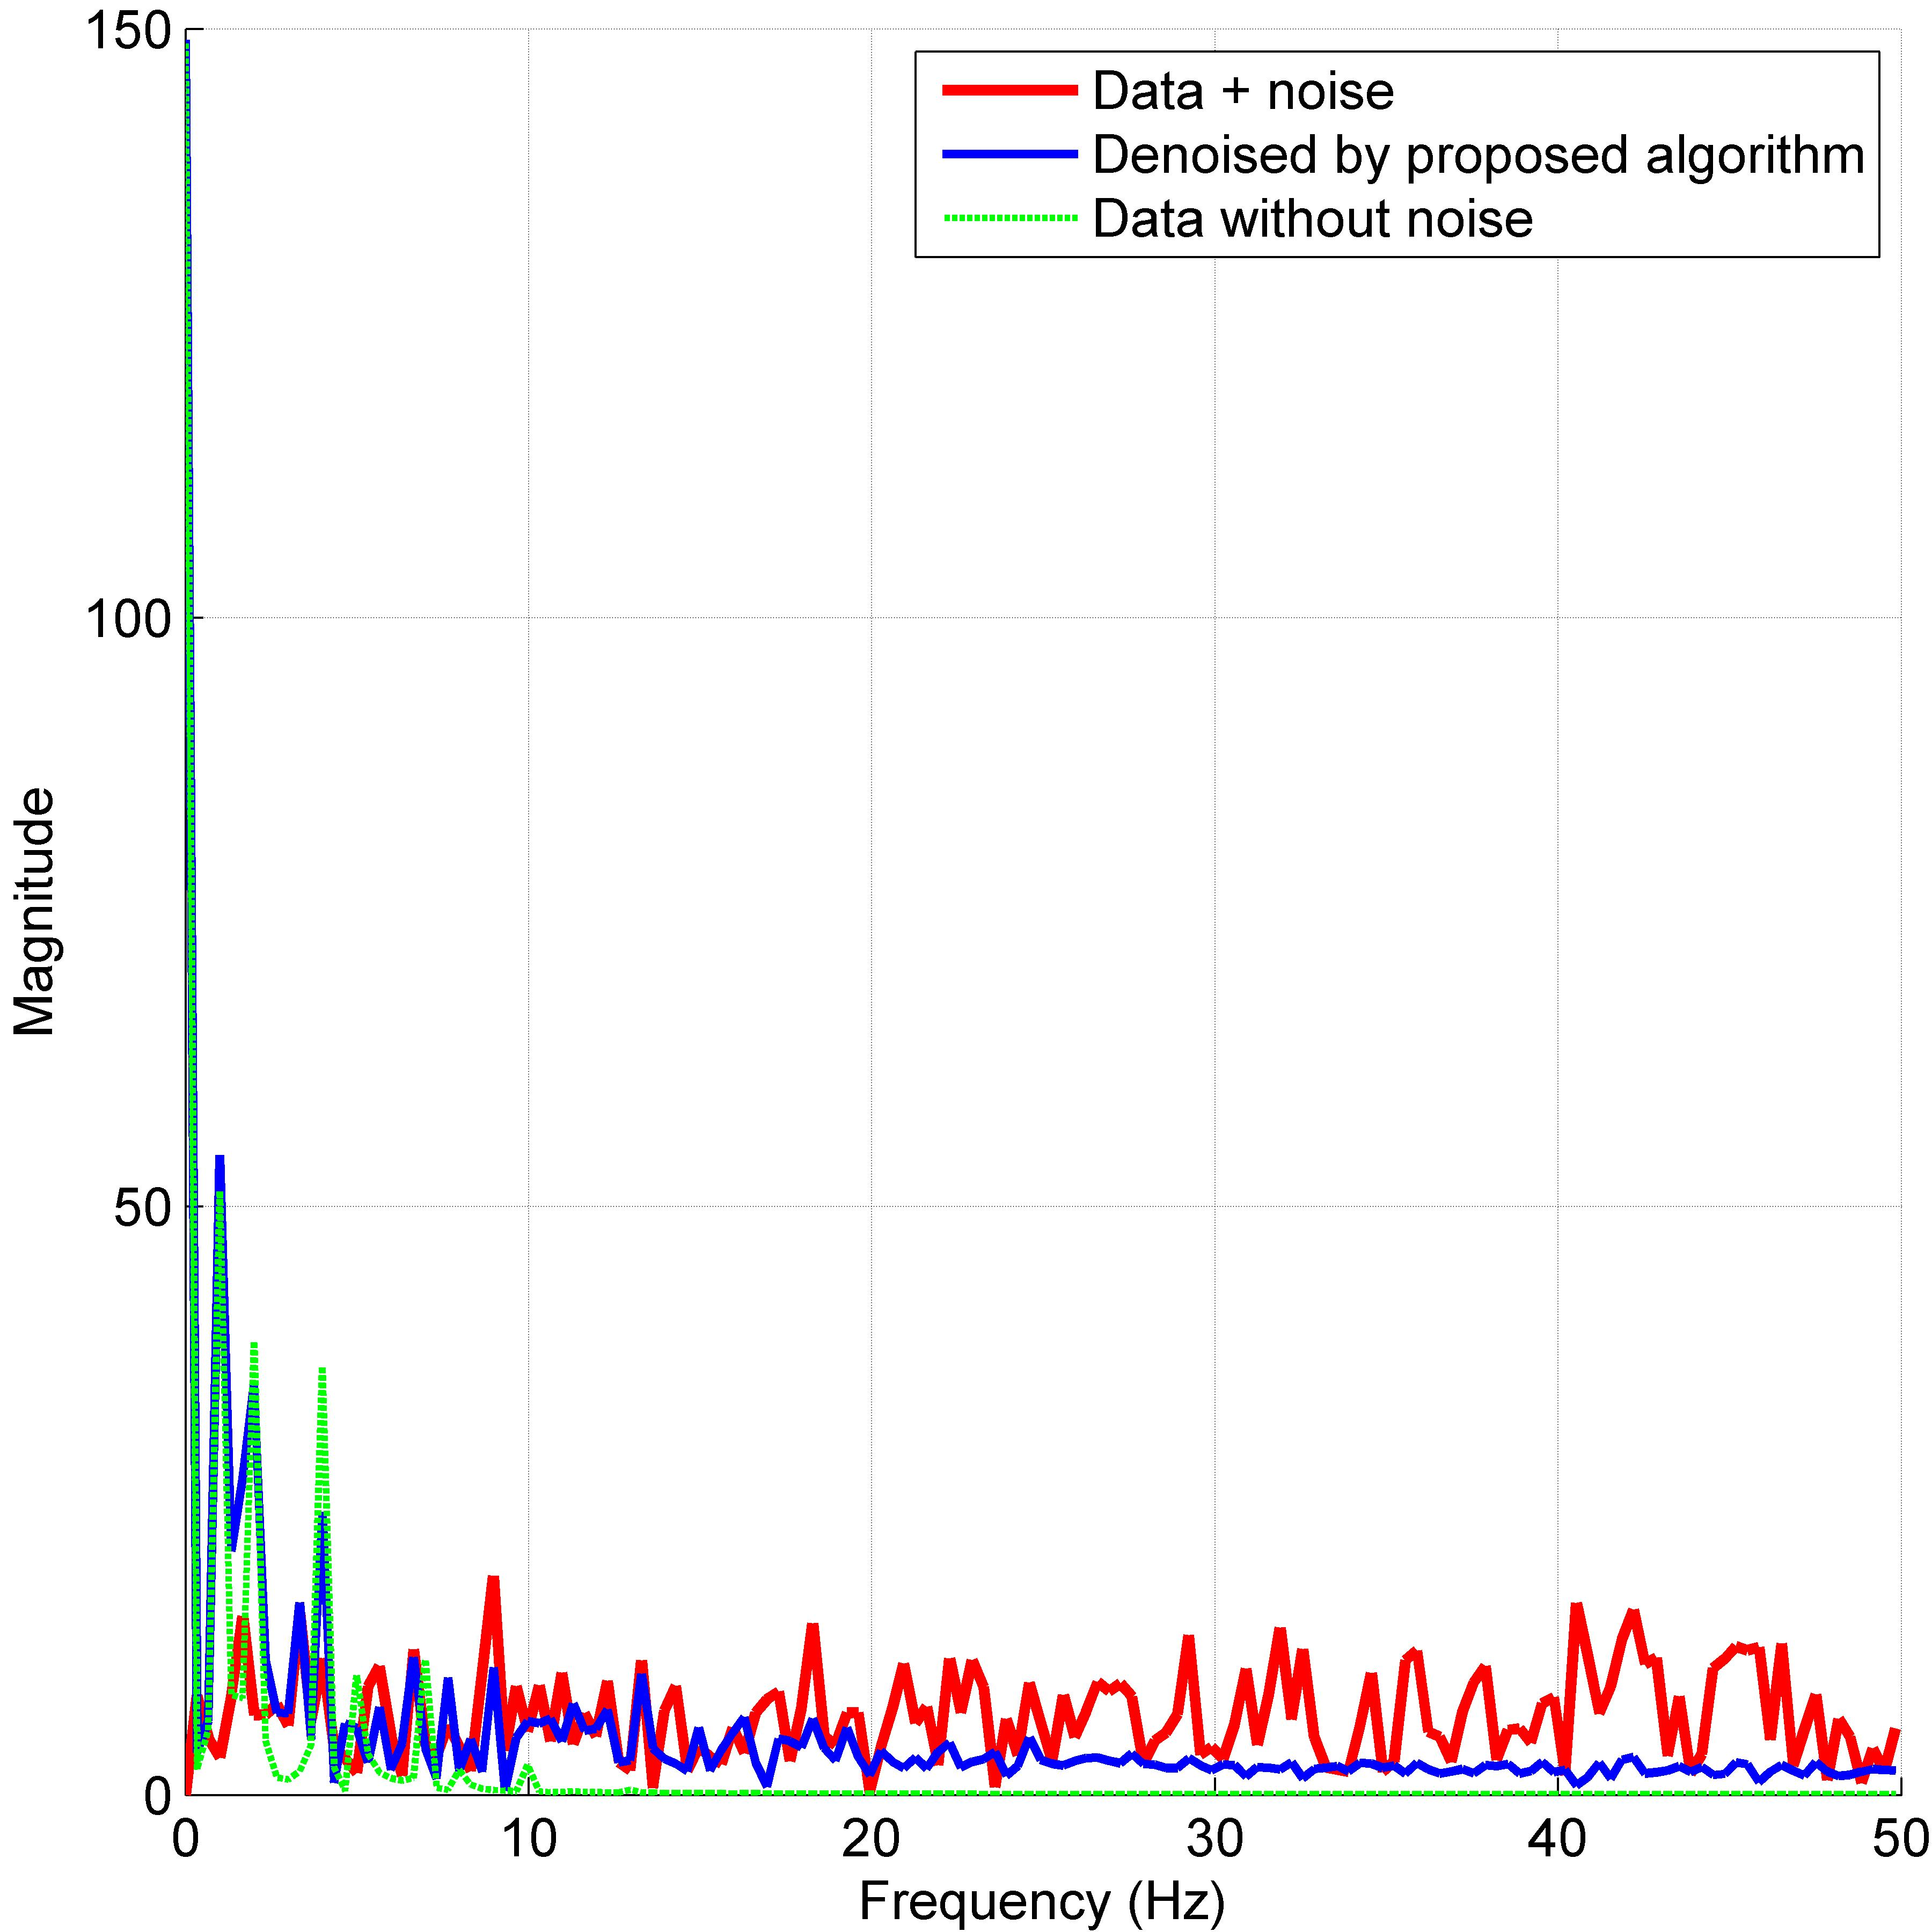
\includegraphics[width=.9\linewidth]{denoise_1.jpg}
  		\caption{\label{fig:denoise_1} Fourier transform of the proposed denoising approach for channel 1.}
	\end{subfigure}%
	\begin{subfigure}{.5\textwidth}
  		\centering
  		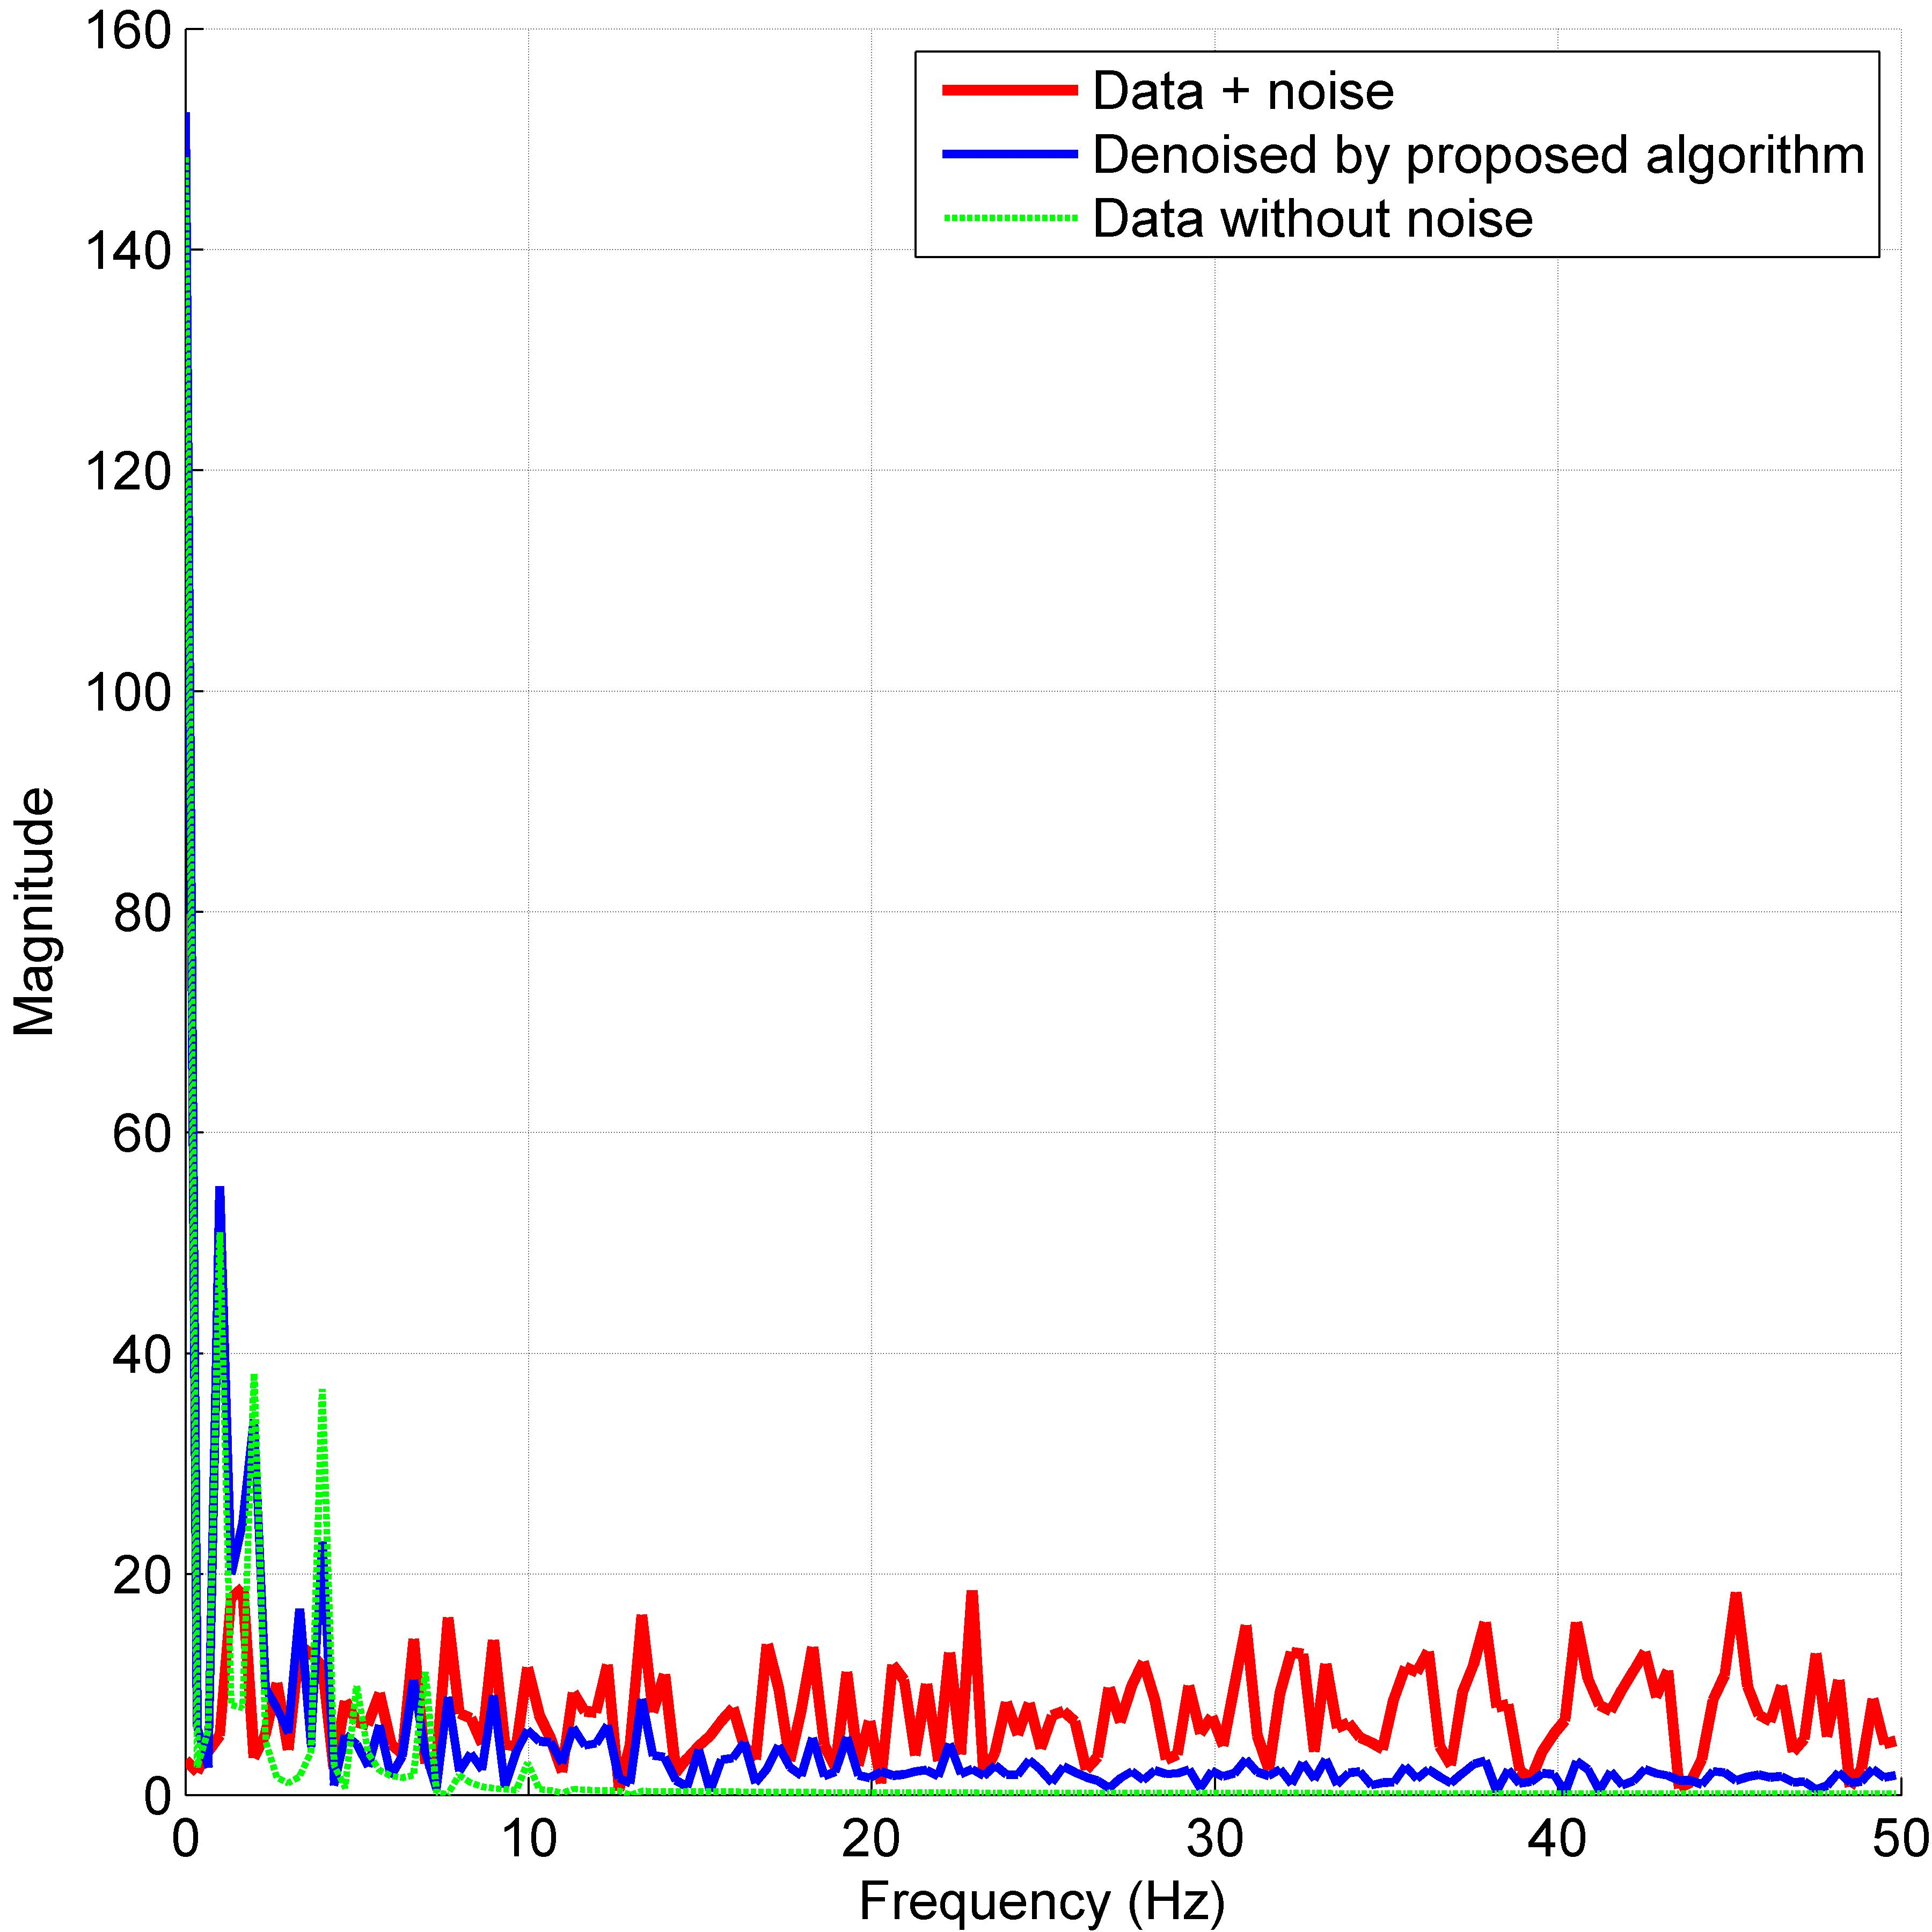
\includegraphics[width=.9\linewidth]{denoise_2.jpg}
  		\caption{\label{fig:denoise_2} Fourier transform of the proposed denoising approach for channel 2.}
	\end{subfigure}
	\caption{Output of the proposed denoising approach on two channels with signals of similar frequency modulation, but shifted in time. This procedure assumes the signal being recorded is from the same source and the noise observed in each channel are correlated.}
\end{figure*}

A fundamental inquiry that needs a resolution is about how the proposed algorithm responds to different SNRs. To address this, the deviations of the Fourier transforms of reconstructed signals as a function of a myriad of SNRs were computed from the Fourier transform of the original signal. These deviation scores were measured as the mean-square errors between the reconstructed signals and the original signal. The threshold employed in this investigation was $99$ percent. From Figure \ref{fig:denoise_3}, it can be noted that the performance of the proposed algorithm increases with an increasing SNR; however, this increase in performance is limited. Since the proposed approach disregards parts of the data that are statistically irrelevant (with respect to the threshold chosen), it is plausible th

\begin{figure*}[ht]
	\centering
	\begin{subfigure}{.5\textwidth}
  		\centering
  		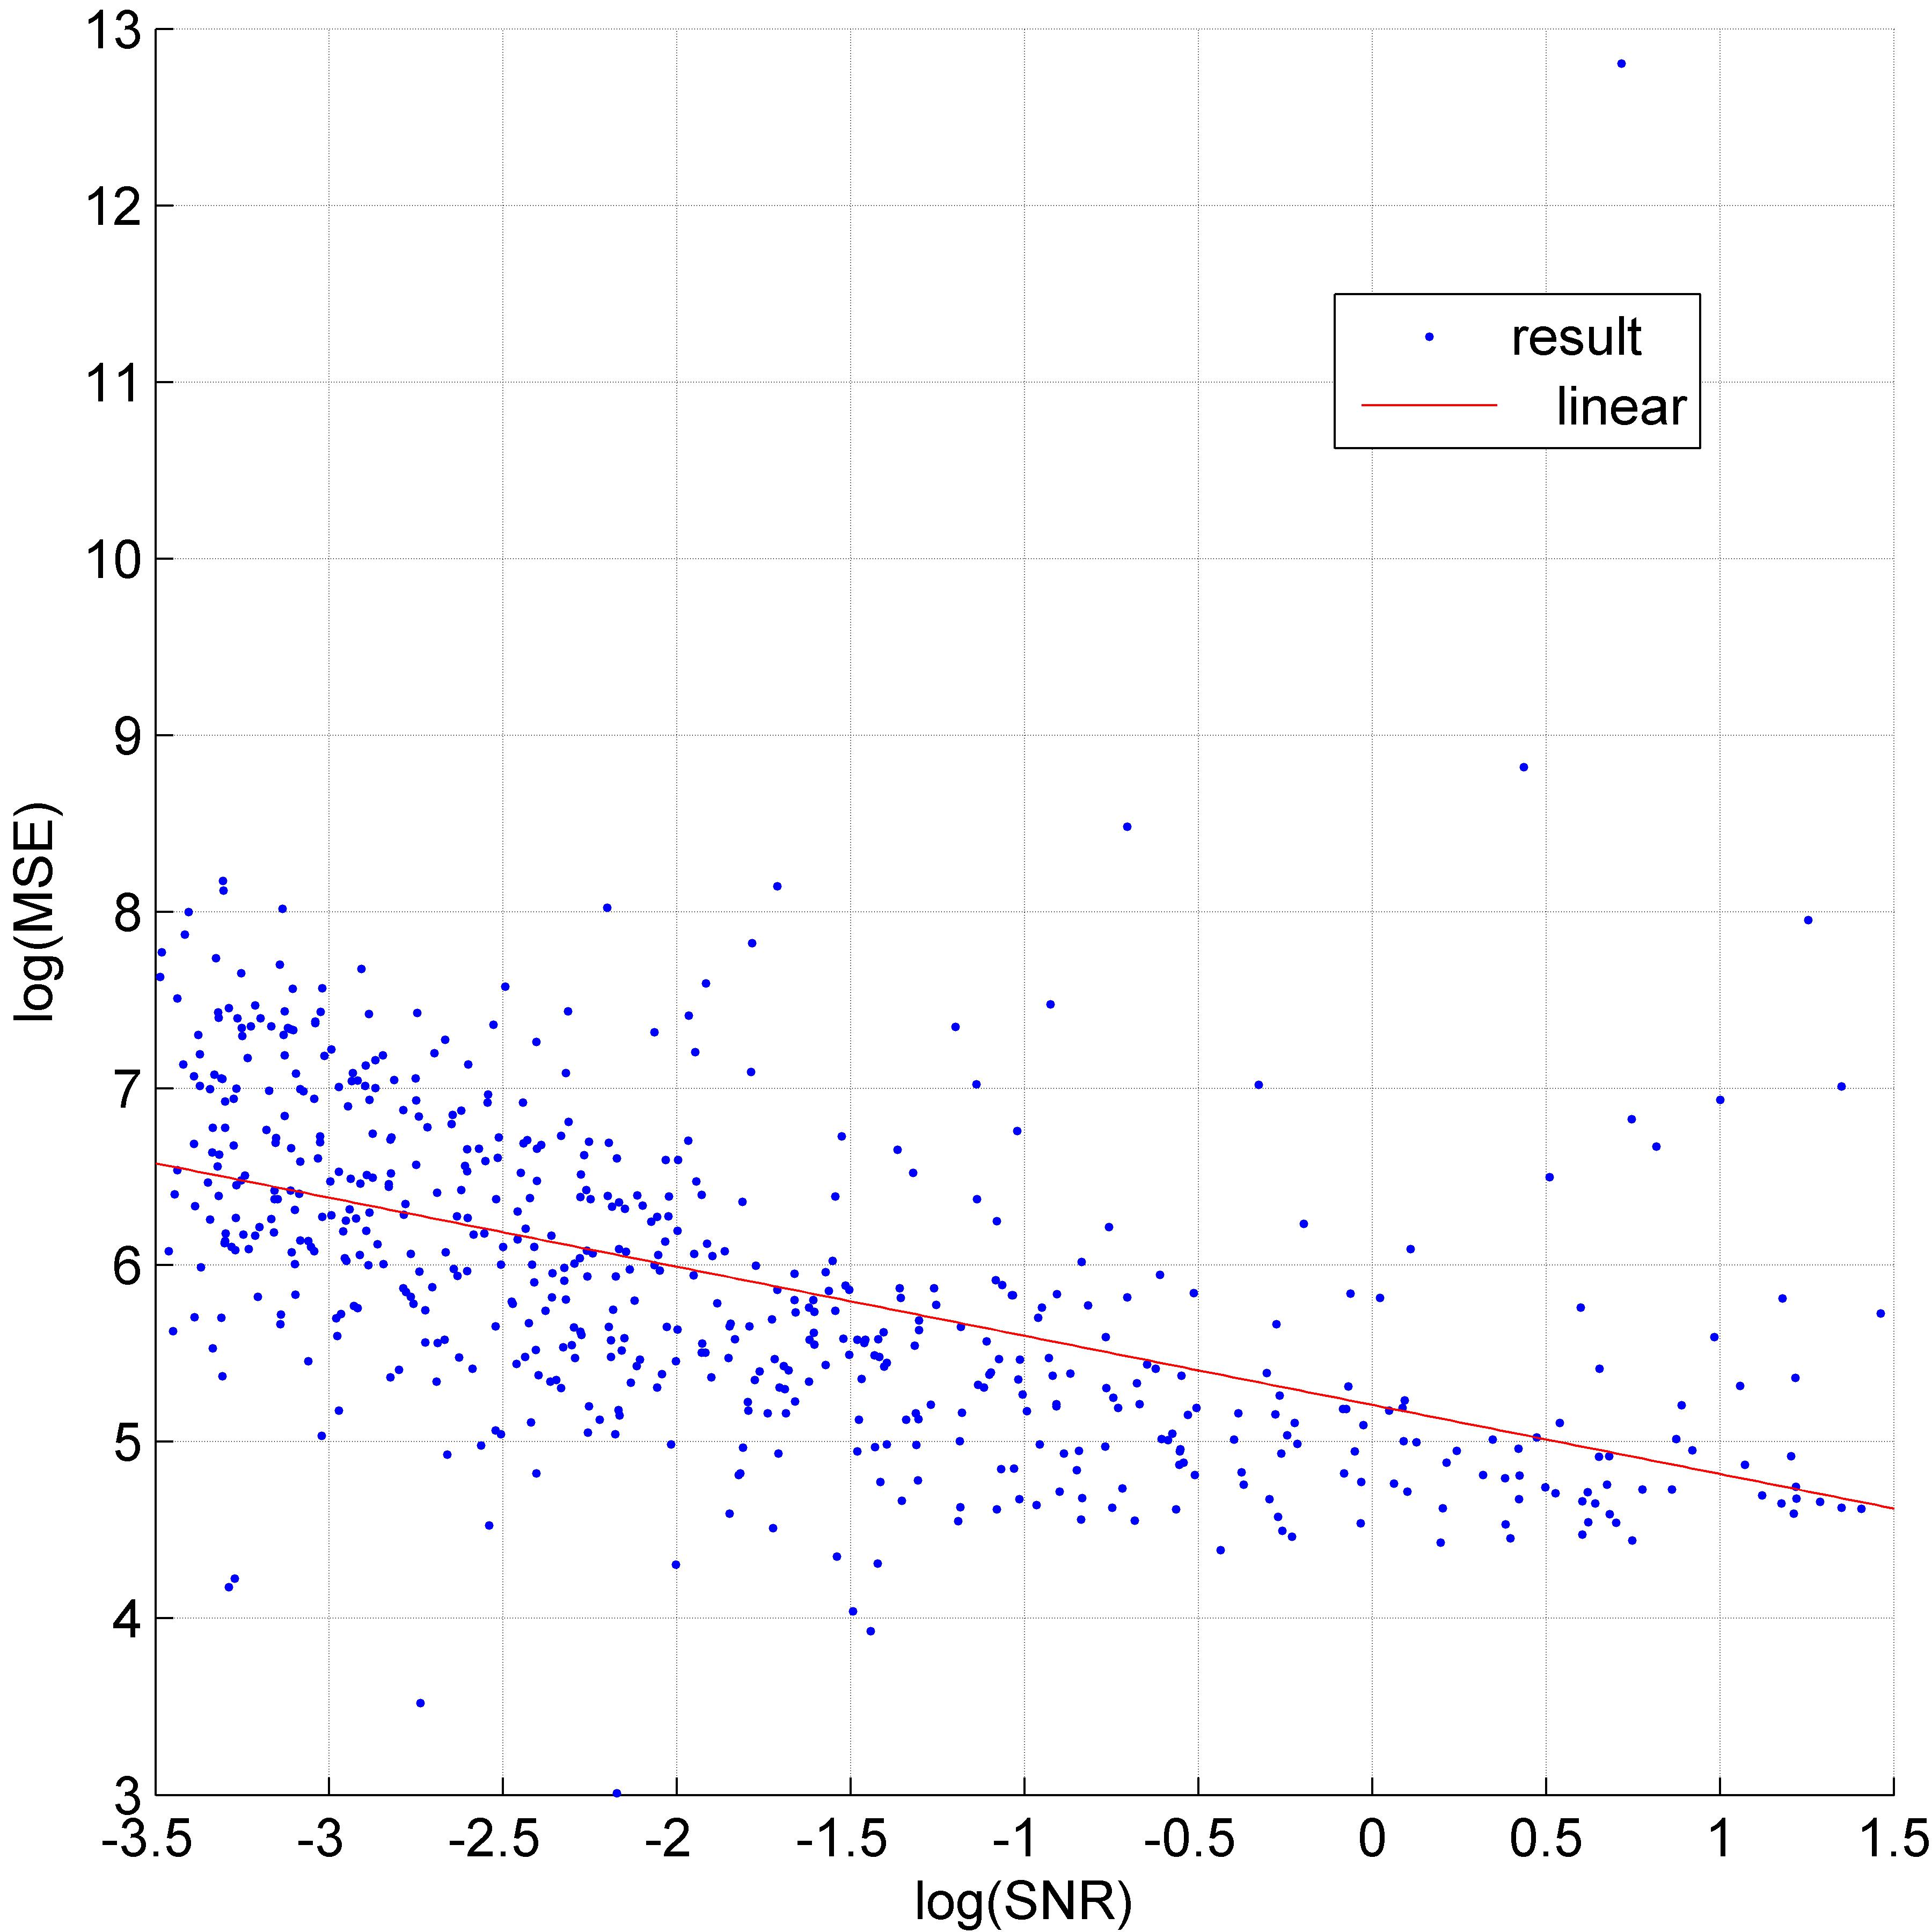
\includegraphics[width=.9\linewidth]{denoise_3.jpg}
  		\caption{\label{fig:denoise_3} Ouput wrt mse and snr}
	\end{subfigure}%
	\begin{subfigure}{.5\textwidth}
  		\centering
  		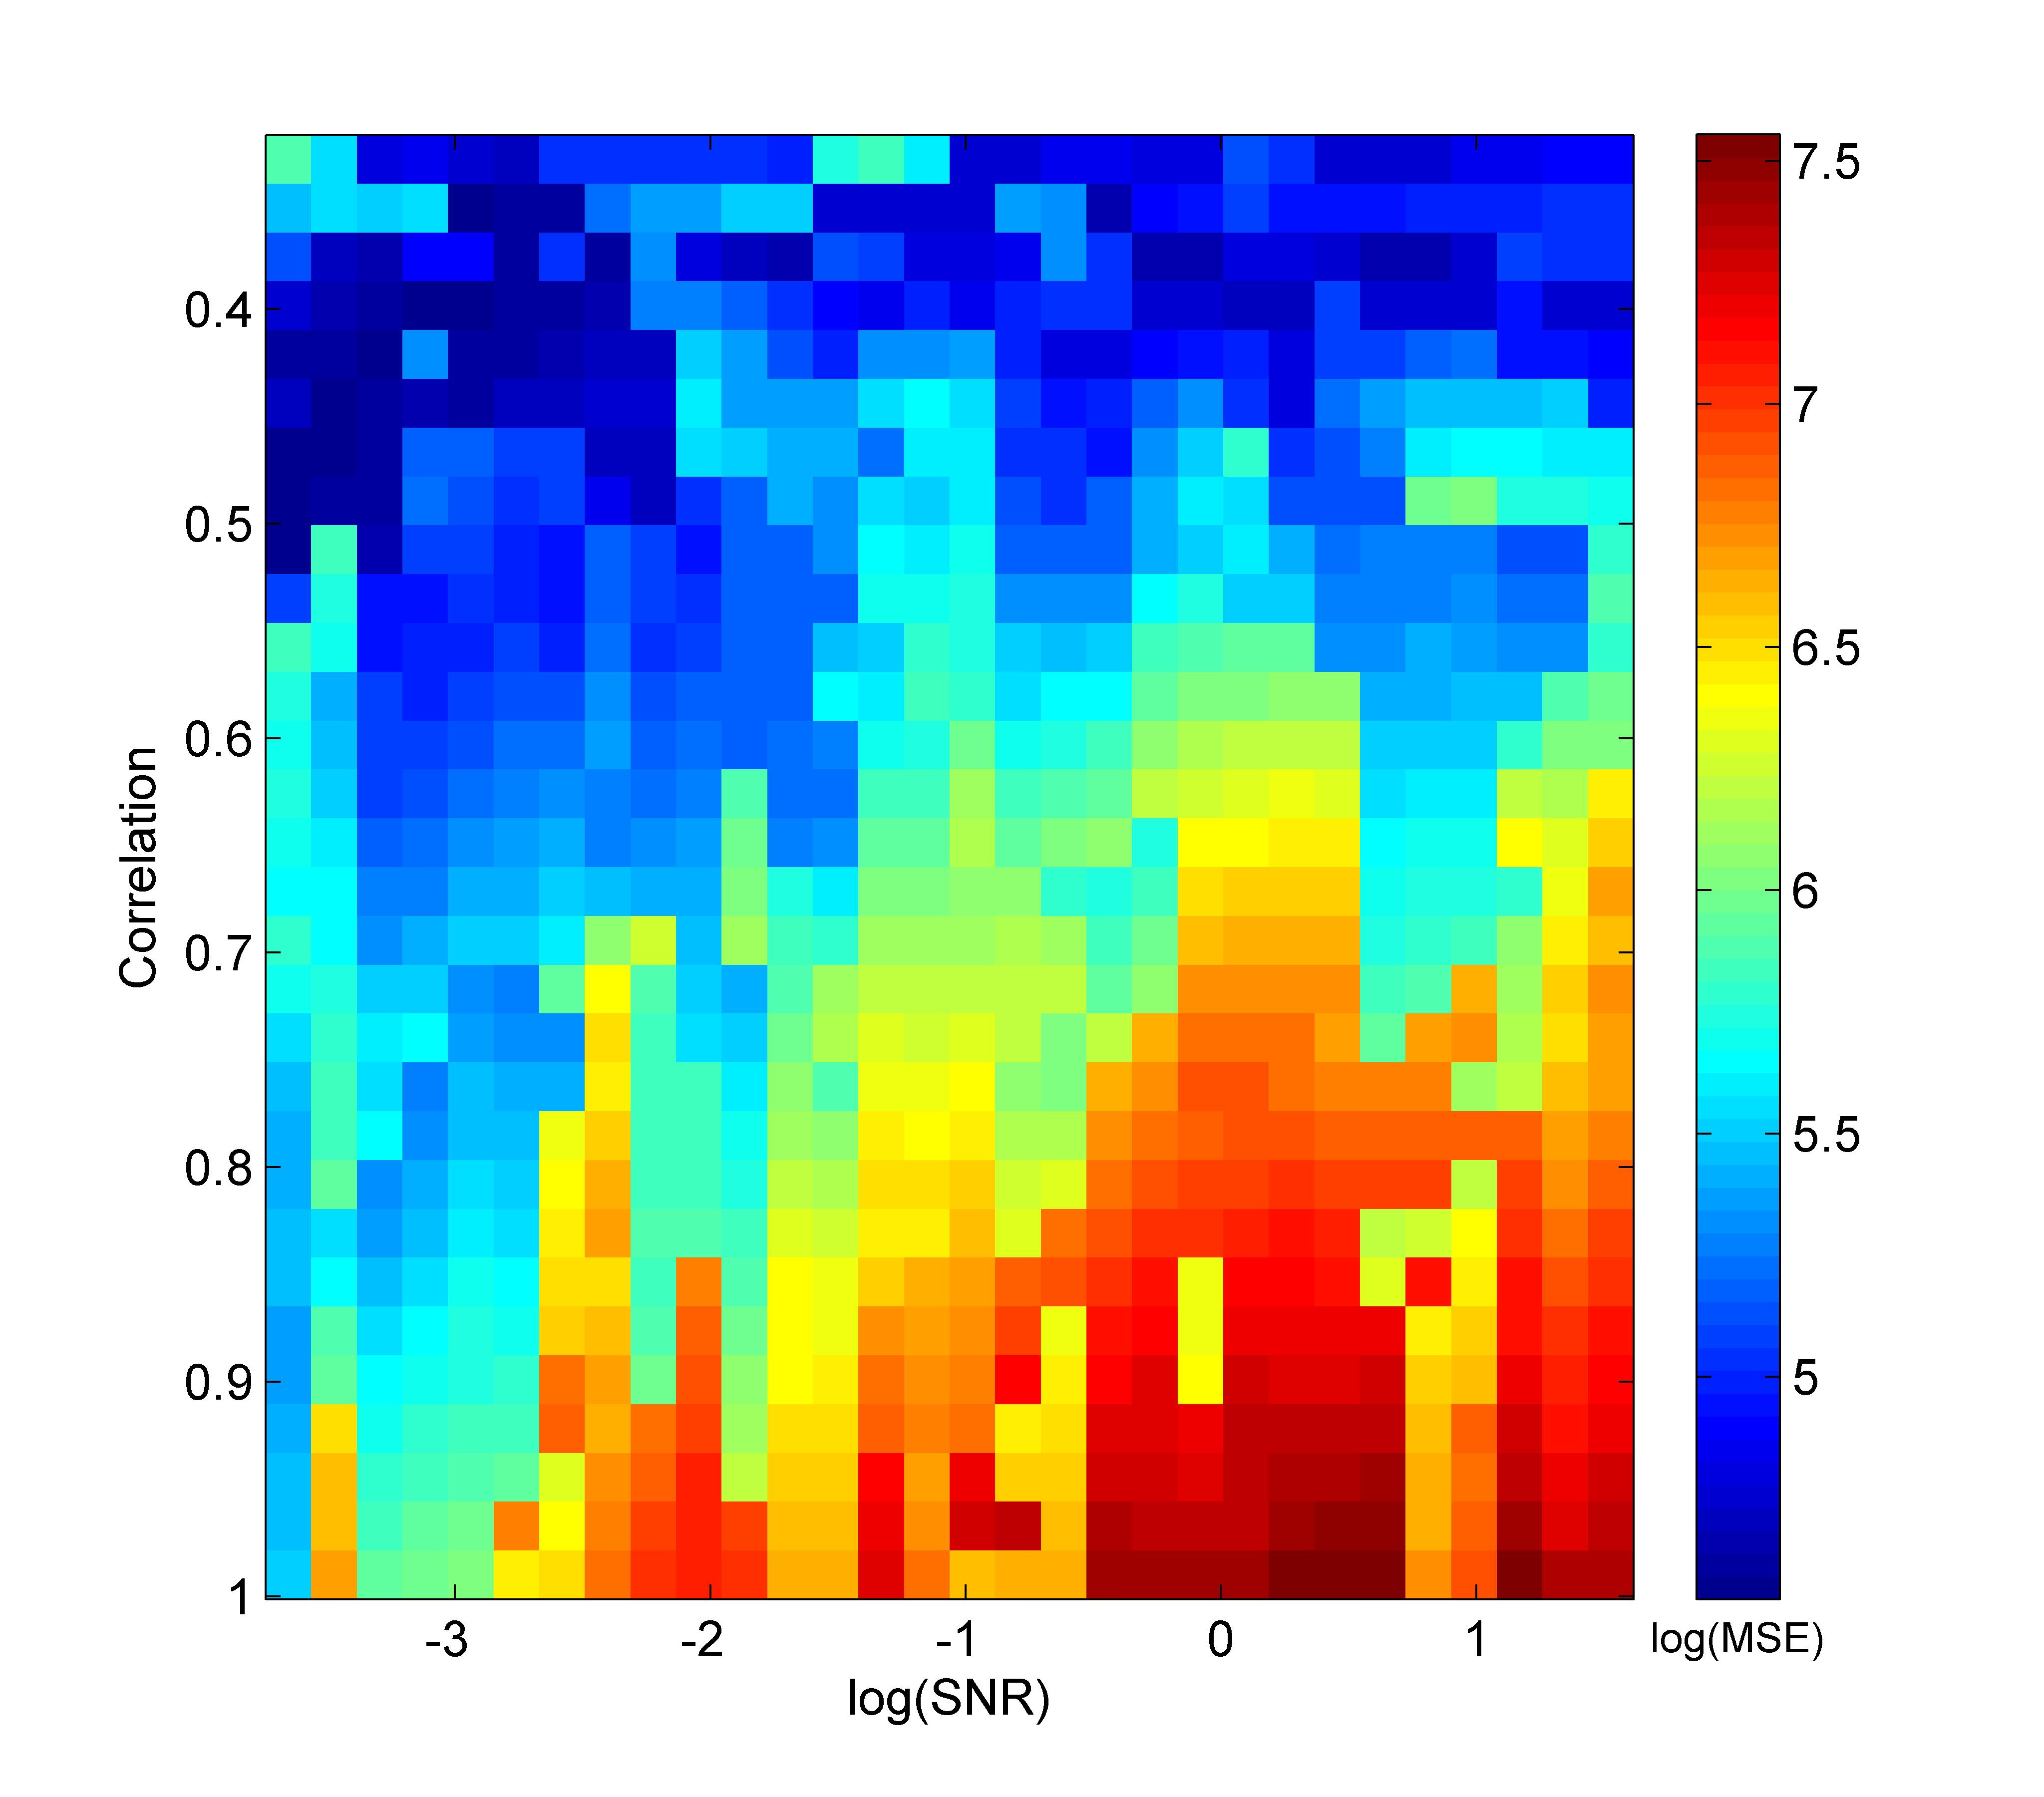
\includegraphics[width=1.15\linewidth]{denoise_4.jpg}
  		\caption{\label{fig:denoise_4} Behaviour of the proposed algorithm under different correlations and SNRs}
	\end{subfigure}
	\caption{Behavior of outputs}
\end{figure*}


\section{Implementing the Gustafson Algorithm in C++}
\subsection{Calculating Bessel Functions}
Known problems with the algorithm include calculating large order bessel functions.  The bessel functions of natural number order are given by

\begin{equation}
J_n(z) = \sum_{m=0}^{\infty} \frac{(-1)^n}{m!(m+n)!} \left( \frac{z}{2} \right)^{2m+n}
\end{equation}

so calculating the nth Bessel function involves calculating factorials greater than n!.  The highest n for which we can store n! in an unsigned long integer type, the largest positive integer type, is 20:

\begin{align}
2^{64}-1 = 18,446,744,073,709,551,615 \\
< 21! = 51,090,942,171,709,440,000
\end{align}

if we are willing to sacrafise some precision to truncation we can use a double precision floating point integer which allows values upto $1.797,693,134,862,315,7 \cdot 10^{308}$

\begin{align}
170! \approx 7.25 \cdot 10^{306}
< 1.797,693,134,862,315,7 \cdot 10^{308} <
171! \approx 1.24 \cdot 10^{309}
\end{align}

This is not acceptable hovever, because $\left| J_n(z) \right| \leq 1$, so when performing the sum we need precision all the way down to at the very least $0.1$, which would require a mantissa with roughly $308$ digits.  This is not only impracticle, but it is by far one of the slowest ways one could calculate values of the Bessel functions.  This whole buiseness of wresteling with factorials can be avoided by calculating the Bessel Functions using Bessel's Equation \ref{eqn:Bessel's Equation} \citep{folland}.

\begin{equation}
\label{eqn:Bessel's Equation}
x^2 J_n''(x) + x J_n'(x) + (x^2 - n^2) J_n(x) = 0
\end{equation}

The standard perscription for numerically solving differential equations is first to discretize the independent variable $x \to x_i = x_{min} + i \cdot \delta x$.  Then use the limit definitions of the derivatives; we will use the three point definitions because their error goes as $O(\delta x^2)$ rather than using the two point definition with an error that goes as $O(\delta x)$ \cite{morten}.  Also, because there are only one order of Bessel Functions in Bessel's Equation, the order is implied by the $n$ that appears, so we will drop the subscript of $n$, $J_n \to J$, and we will further adopt the notation $J(x_i) = J_i$.

\begin{align}
J_i'  &= \frac{J_{i+1} - J_{i-1}}{2 \delta x} \\
J_i'' &= \frac{J_{i-1} - 2J_{i} + J_{i+1}}{\delta x^2}
\end{align}

So the discretized form of Bessel's Equation is

\begin{align}
\label{eqn:Bessel's Equation Discretized}
x_i^2 \frac{J_{i-1} - 2J_{i} + J_{i+1}}{\delta x^2} + x \frac{J_{i+1} - J_{i-1}}{2 \delta x} + (x^2 - n^2) J_i = 0
\end{align}

\begin{align}
\left(\frac{x_i^2}{\delta x^2} - \frac{x_i}{2\delta x}\right) J_{i-1}
	+ \left( \left(1-\frac{2}{\delta x^2}\right)x_i^2 - n^2 \right) J_i
	+ \left(\frac{x_i^2}{\delta x^2} + \frac{x_i}{2\delta x}\right) J_{i+1}
	= 0
\end{align}

Where we have collected like terms of $J_i$.  For convenience we define coefficients to simplify the above equation.

\begin{align}
a_i &= \frac{x_i^2}{\delta x^2} - \frac{x_i}{2\delta x} 	\\
b_i &= \left(1-\frac{2}{\delta x^2}\right)x_i^2 - n^2  	\\
c_i &= \frac{x_i^2}{\delta x^2} + \frac{x_i}{2\delta x}
\end{align}

These coefficients can be simplified by using the definition for $x_i$, and taking $x_{min} = 0$.

\begin{align}
a_i &= i   \left( i - \frac{1}{2} \right)				\\
b_i &= i^2 \left( \delta x^2 - 2  \right) - n^2 		 	\\
c_i &= i   \left( i + \frac{1}{2} \right)
\end{align}

So the discretized Bessel equation with simplified coefficients is

\begin{align}
a_i J_{i-1} + b_i J_i + c_i J_{i+1} = 0
\end{align}

Wrighting out the system of equations explicitly:

\begin{align}
b_1 J_1 + c_1 J_2                                 &= - a_1 J_0		\\
a_2 J_1 + b_2 J_2 + c_2 J_3                       &= 0				\\
a_3 J_2 + b_3 J_3 + c_3 J_4                       &= 0				\\
                                                  &\vdots				\\
a_{n-1} J_{n-2} + b_{n-1} J_{n-1} + c_{n-1} J_{n} &=   0				\\
a_n J_{n-1} + b_n J_n                             &= - c_n J_{n+1}
\end{align}

Which suggests Bessel Equation be written as a matrix equation.

\begin{align}
\left( \begin{array}{ccccc}
	b_1 & c_1 &         &         &         \\
	a_2 & b_2 &   c_2   &         &         \\
	    & a_3 &   b_3   &   c_3   &         \\
	    &     & \vdots  & \vdots  &         \\
	    &     & a_{n-1} & b_{n-1} & c_{n-1} \\
	    &     &         &   a_n   &   b_n
\end{array} \right)
\left( \begin{array}{c}
	  J_1   \\
	  J_2   \\
	  J_3   \\
	\vdots  \\
	J_{n-1} \\
	  J_n
\end{array} \right)
=
\left( \begin{array}{c}
	  - a_1 J_0   \\
	      0       \\
	      0       \\
	   \vdots     \\
	      0       \\
	- c_n J_{n+1}
\end{array} \right)
\end{align}

This is a tridiagonal matrix system that charactorized a one dimentional differential equation.  It can be easilly solved using the standard Thomas Algorithm.  To program this in C++ we need all the arrays to be indexed from 0, so 

\begin{align}
\label{eqn:finalDiscretizedBesselMatrixEqn}
\left( \begin{array}{ccccc}
	B_0 & C_0 &         &         &         \\
	A_1 & B_1 &   C_1   &         &         \\
	    & A_2 &   B_2   &   C_2   &         \\
	    &     & \vdots  & \vdots  &         \\
	    &     & A_{N-4} & B_{N-4} & C_{N-4} \\
	    &     &         & A_{N-3} & B_{N-3}
\end{array} \right)
\left( \begin{array}{c}
	  J_1   \\
	  J_2   \\
	  J_3   \\
	\vdots  \\
	J_{N-3} \\
	J_{N-2}
\end{array} \right)
=
\left( \begin{array}{c}
	    - A_0 J_0     \\
	        0         \\
	        0         \\
	     \vdots       \\
	        0         \\
	- C_{N-3} J_{N-1}
\end{array} \right)
\end{align}

\begin{align}
A_i = a_{i+1} &= (i+1)   \left( i + \frac{1}{2} \right)				\\
B_i = b_{i+1} &= (i+1)^2 \left( \delta x^2 - 2  \right) - n^2			\\
C_i = c_{i+1} &= (i+1)   \left( i + \frac{3}{2} \right)
\end{align}

\subsubsection{The Thomas Algorithm}
The Thomas Algorithm is a lightning fast way to solve tridiagonal systems like equation \ref{eqn:finalDiscretizedBesselMatrixEqn}.  The algorithm consists of two steps.  First there is a forward substitution which eliminates the $A_i$'s, and modifies the $B_i$'s and the vector on the right which we will call the source vector $S_i; \quad \forall i \in [0, N-3]$.

\begin{align}
R_i &=   R_i - \frac{A_i}{B_{i-1}} R_{i-1}; 	\qquad \forall i \in [1, N-3]		\\
B_i &\to B_i - \frac{A_i}{B_{i-1}} C_{i-1}; 	\qquad \forall i \in [1, N-3]		\\
S_i &\to S_i - \frac{A_i}{B_{i-1}} S_{i-1}; 	\qquad \forall i \in [1, N-3]
\end{align}

Then there is a backwards substitution eliminating the $C_i$'s, again modifying the $S_i$'s.  Finally we solve for $J_i$.

\begin{align}
R_i &=   R_i - \frac{C_i}{B_{i+1}} R_{i+1}; \qquad \forall i \in [N-4, 0]	\\
S_i &\to S_i - \frac{C_i}{B_{i+1}} S_{i+1}; \qquad \forall i \in [N-4, 0]	\\
J_i &=   \frac{S_{i-1}}{B_{i-1}};           \qquad \forall i \in [N-2, 1]
\end{align}

The time it takes to perform the Thomas Algorithm goes as $N$ \cite{}.



\subsubsection{Boundary Conditions \label{sec:boundaryConditions}}

To solve this second-order differential equation we will need two boundary conditions.  The boundary condition at $x=0$ is simple.

\begin{displaymath}
   J_n(0) = \left\{
     \begin{array}{lr}
       1 & : n = 0     \\
       0 & : n \neq 0
     \end{array}
   \right.
\end{displaymath}

For the other boundary condition we \textit{could} use the asymtotic form of the Bessel functions.  Theorem 5.1 in \cite{folland} states:

\textit{For each $n \in N$ there is a constant $C_n \in R$ such that, if $x \geq 1$, then}

\begin{equation}
\label{eqn:asymtoticBessel}
\left| J_n(x) - \sqrt{\frac{2}{\pi x}} \cos \left( x - \frac{\pi}{4} (2n+1) \right) \right| \leq \frac{C_n}{x^{3/2}}
\end{equation}

This is an asymptotic expansion, so it is only valid for large values of x.  It turns out the accuracy of the solution to bessels equation relies heavilly on the accuracy of the endpoint at $x \neq 0$.  Figures \ref{fig:BesselBadBoundary} and \ref{fig:BesselGoodBoundary} illistrate this point quite well.  The conclusion is that the asymtotic form of the bessel functions is not accurate enough for even fairly large valuse of $z$.  We can also do

\begin{align}
J_n (z) = \frac{1}{\pi} \int_{0}^{\pi} \cos \left[ z \sin \theta - n \theta \right] d \theta
\end{align}

Which is computed using a Riemann Sum

\begin{align}
\label{eqn:numericalIntegralBessel}
J_n (z) &\approx \frac{1}{N} \sum_{i=0}^{N+1} \cos \left[ z \sin(i \cdot dx) - n \cdot i \cdot dx \right];
\qquad dx = \frac{\pi}{N}
\end{align}

The function being integrated becomes more oscillitory as $n$ increases.  Numerical analysis shows that $n$ gives the number of zeros the function has  on the interval $(0,\pi)$ for $z=0$.  For $n=0$ the number of zeros is given by $Floor (\frac{2z}{\pi})$.  We want a way to ensure the calculation is accurate regardless of how oscillatory it is, but we also want it to be as fast as possible, so we use these facts regarding the zeros to ensure there are roughly the same number of integration points between zeros.  By taking the number of (evenly spaced) integration points to be

\begin{align}
\label{eqn:dynamicIntegrationPoints}
N = 100 \cdot (n + 1) \cdot Floor \left( \frac{2z}{\pi} + 1 \right)
\end{align}

we acheved excellent results (accurate consistantly to 16 decimal places) for a wide range of $z$ and $n$.  The $+1$'s are to ensure accurate results when $z$ or $n$ are zero.  The algorithm can have problems when $J$ is extremely small.  Then the function can be off by many orders of magnitude, but because it is essentially zero, it does not seem to effect our results when used as a boundary condition for solving Bessel's Differential Equation.

\begin{figure*}[t]
	\centering
	\begin{subfigure}{.5\textwidth}
  		\centering
  		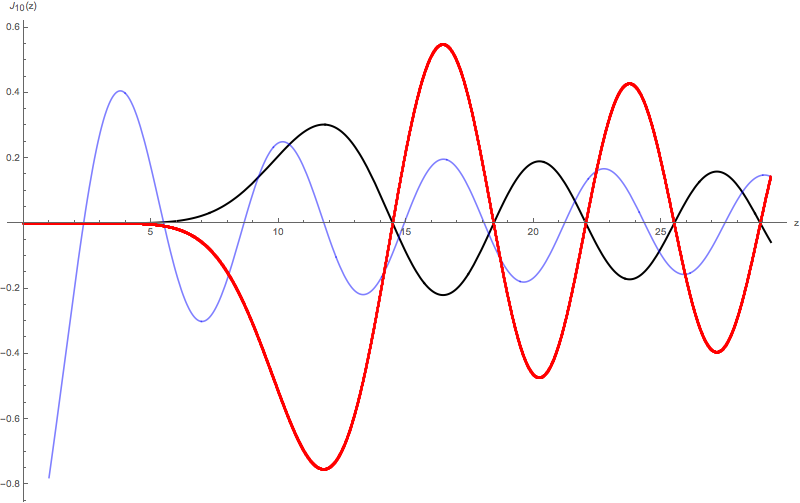
\includegraphics[width=.9\linewidth]{BesselBadBoundary.png}
  		\caption{\label{fig:BesselBadBoundary} Notice how the asymtotic form and the one calculated by our differential equation solver match up at the maximum value for $z$, but do not match up with the true solution.  This has far reaching consequences.  Whatever multiplicative factor the endpoint is off by seems to carry through for every other point.  In this case the multiplicative factor (asymtotic / true) is almost exactly $-2.5$.  Notice how this inverts the solution and makes it $250\%$ larger.}
	\end{subfigure}%
	\begin{subfigure}{.5\textwidth}
  		\centering
  		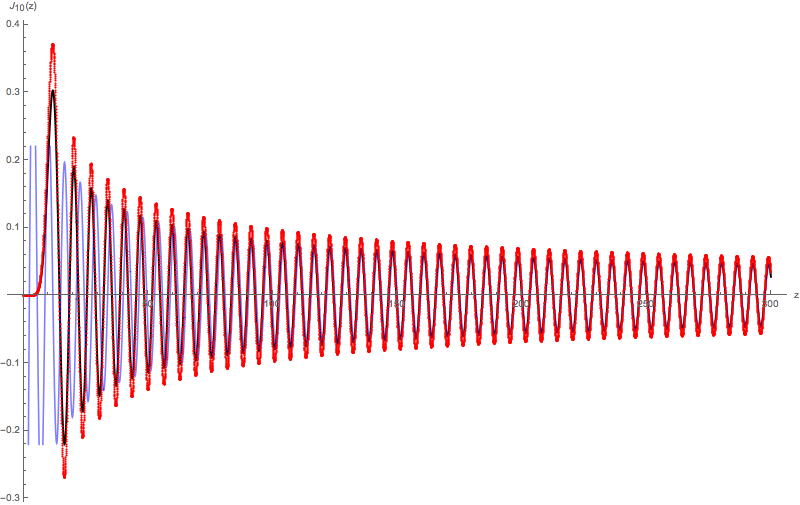
\includegraphics[width=.9\linewidth]{BesselGoodBoundary.png}
  		\caption{\label{fig:BesselGoodBoundary} For much larger values of $z$ the asymtotic form is a better approximation to the true value.  In this case the multiplicative factor (asymtotic / true evaluated at $z=300$) is roughtly $1.2$ which results in the soultion being roughly $20\%$ larger than it should be.}
	\end{subfigure}
	\caption{The blue curve is the asymtotic form of the bessel functions as given in equation \ref{eqn:asymtoticBessel}, the black curve is $J_{10} (x)$ as given by Mathematica, and the red curve is the one calculated by our differential equation solver.  Note, both of these solutions were calculated using 10,000 points.  Even though the solution in figure \ref{fig:BesselBadBoundary} has 10 times the point density, it is limited in accuracy by the endpoint!}
\end{figure*}

\subsubsection{Calculating Bessel Functions: Results}
The ultimate benchmark for sucess in calculating Bessel Functions in this manner (using the Thomas Algorithm to solve Bessel's Differential Equation) is to compare it to the stardard way of calculating the value at each point using the Riemann Sum (as defined in equation \ref{eqn:numericalIntegralBessel} section \ref{sec:boundaryConditions}).  So how much faster is it?  This depends on the values of $n$ and $z$ because we use a dynamic number of integration points as given by eq. \ref{eqn:dynamicIntegrationPoints}. Table \ref{table:besselSpeed} gives the speed increse for various parameters.

\begin{table*}[t]
	\centering
	\begin{tabular}{l || c | c | c }
		                  & Point by Point & Thomas Algo. Solving &  Speed	\\
		Parameters        & Using Integral &  Bessel's Equation   & Increse	\\
		\hline
		\hline
		n = 3             &   0.051786 s   &      0.00013800 s    &   375		\\
		N = 500           &                &                      &			\\
		$z_{max} = 20.0$  &                &                      &			\\
		\hline
		n = 14            &     113.33 s   &       0.003937 s     & 28,785	\\
		N = 50,000        &                &                      &           \\
		$z_{max} = 100.0$ &                &                      &           \\
	\end{tabular}
	\caption{\label{table:besselSpeed} $N$ is the number of points returned, $n$ is the order of the bessel function, and the points calculated were for $z \in [0,z_{max}]$ }
\end{table*}

Table \ref{fig:selectBesselFunctions} gives three examples of Bessel Functions that were calculated using the Thomas Algorithm to solve Bessel's Equation.

\begin{figure*}[t]
	\centering
	\begin{subfigure}{.5\textwidth}
  		\centering
  		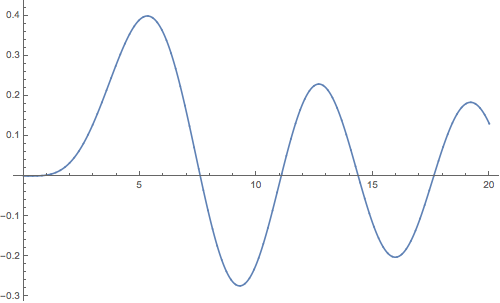
\includegraphics[width=.9\linewidth]{BesselJ4.png}
  		\caption{n=4, numPts=10,000, xMax=20, comptime=0.00082}
	\end{subfigure}%
	\begin{subfigure}{.5\textwidth}
  		\centering
  		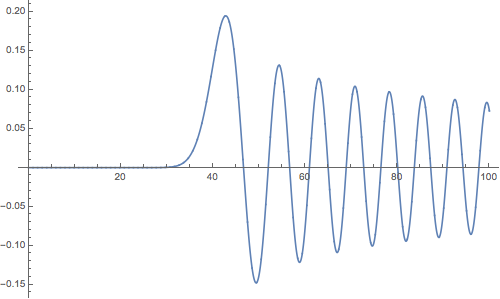
\includegraphics[width=.9\linewidth]{BesselJ40.png}
  		\caption{n=40, numPts=10,000, xMax=100, comptime=0.00092}
	\end{subfigure}
	\begin{subfigure}{.5\textwidth}
  		\centering
  		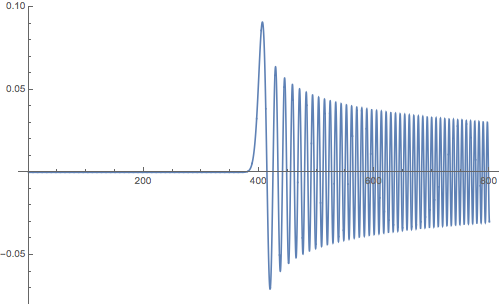
\includegraphics[width=.9\linewidth]{BesselJ400.png}
  		\caption{n=400, numPts=10,000, xMax=800, comptime=0.00200;  About half the computation time went to calculating the endpoint!}
	\end{subfigure}
	\caption{\label{fig:selectBesselFunctions}}
\end{figure*}


\begin{figure*}[t]
	\centering
	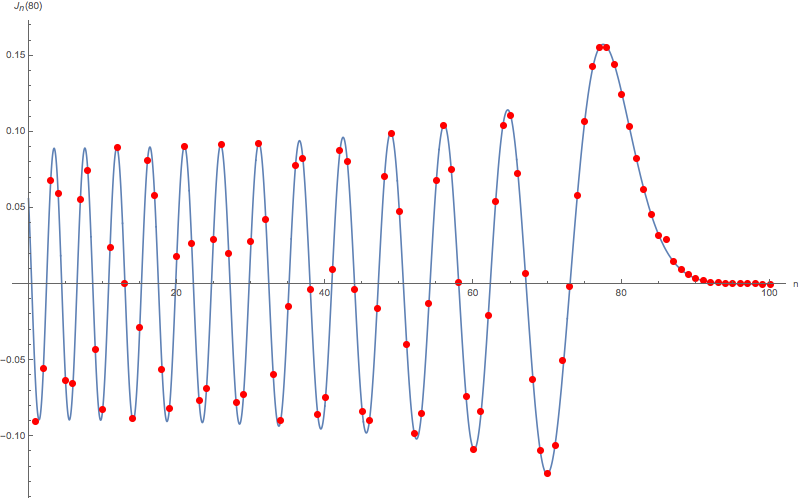
\includegraphics[width=.75\linewidth]{BesselJn80.png}
	\caption{This plot is a plot of $J_n(80)$ for values of $n\in (0,100)$.  The blue curve was generated by the BesselJ function of Mathematica.  The red dots were calculated by my code.  The two sets of data are in excelent agreement at except perhaps $n=0,85$ in which case there is a slight disagreement.  This is a small selection of the $400,000$ data points my code generated in $0.33$ seconds (on 5 year old a loptop).  It solved the Bessel differential equation for $4000$ steps in $\Gamma \in (0,100)$, then saves the output, and moved on to solve Bessel's Equation for the next value of n until all values of $\Gamma$ and n were solved for.}
\end{figure*}


\section{C++ Implementation of the Gustafson Algorithm: Results}
-Step size in omega0 and omega1 must be small because they are deltas.
-Step size in phi1 can be larger because it is less sharply peaked.
-Step size in Gamma can be even larger because it is relatively smooth.

\begin{figure*}[t]
	\centering
	\begin{subfigure}{.5\textwidth}
  		\centering
  		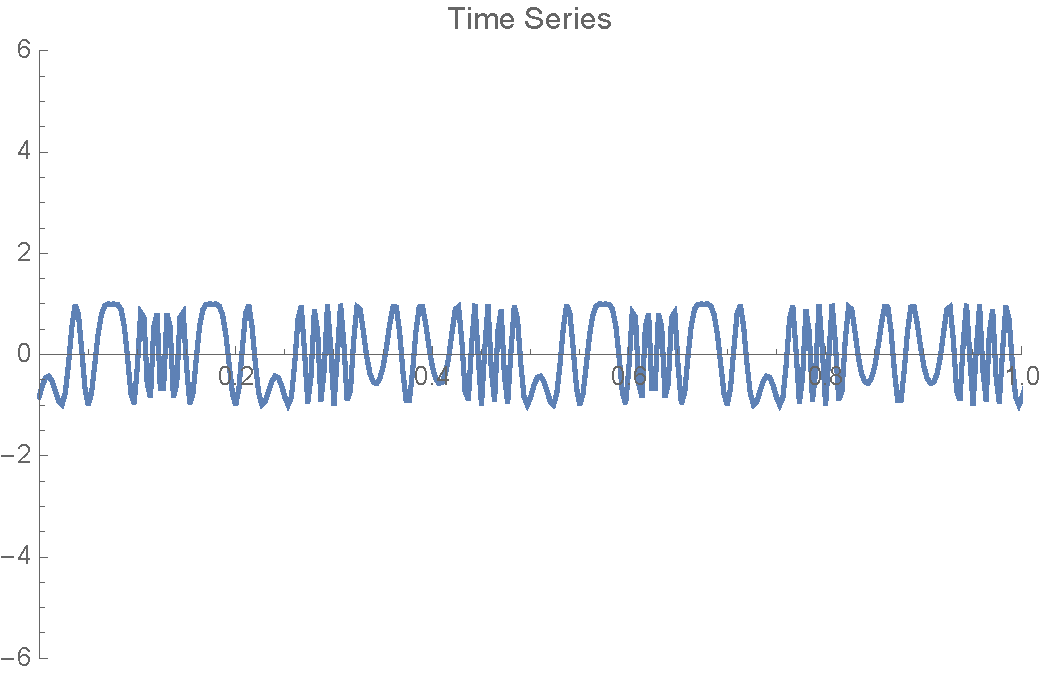
\includegraphics[width=.9\linewidth]{timeSeries.pdf}
  		\caption{}
	\end{subfigure}%
	\begin{subfigure}{.5\textwidth}
  		\centering
  		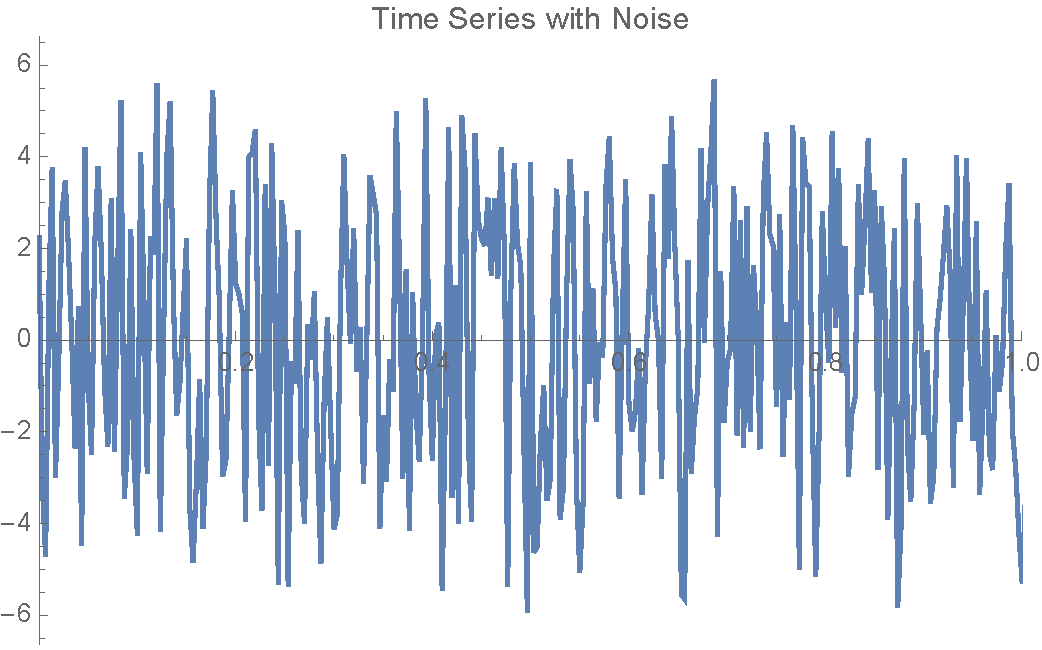
\includegraphics[width=.9\linewidth]{timeSeriesNoise.pdf}
  		\caption{}
	\end{subfigure}
	\begin{subfigure}{.5\textwidth}
  		\centering
  		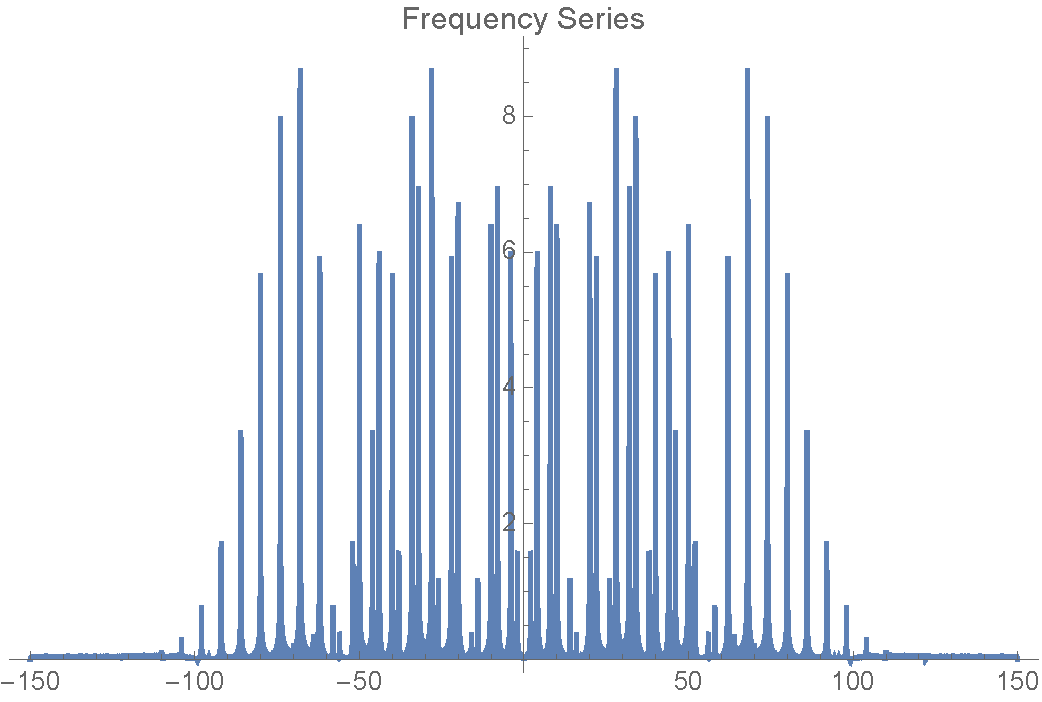
\includegraphics[width=.9\linewidth]{fourierSeries.pdf}
  		\caption{}
	\end{subfigure}%
	\begin{subfigure}{.5\textwidth}
  		\centering
  		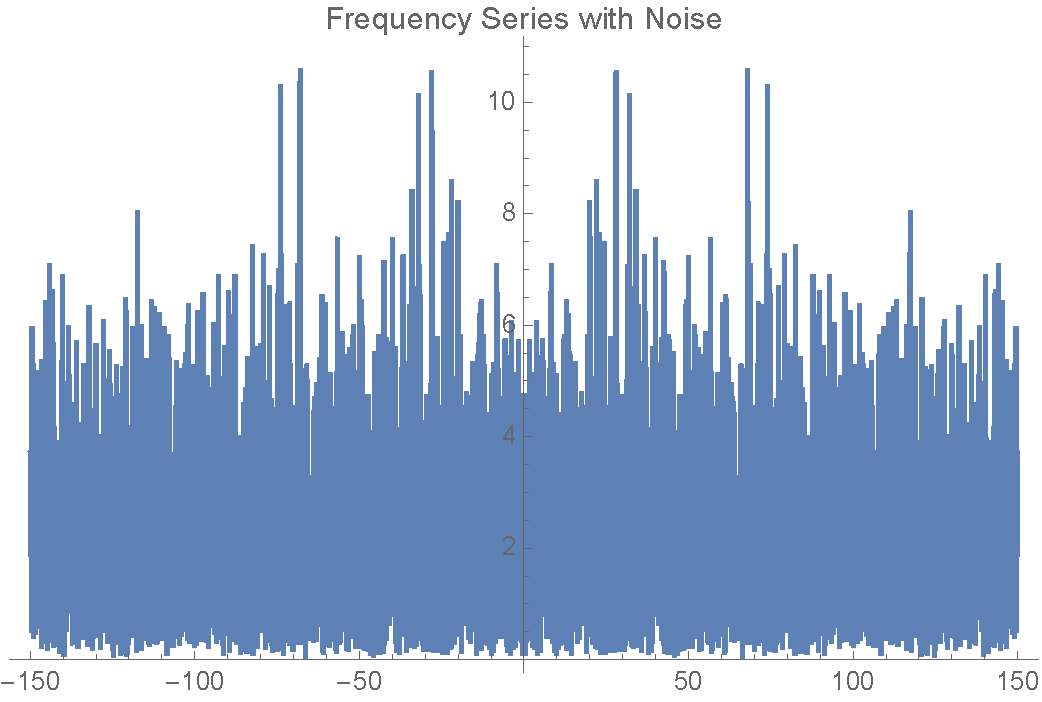
\includegraphics[width=.9\linewidth]{fourierSeriesNoise.pdf}
  		\caption{}
	\end{subfigure}
	\begin{subfigure}{.5\textwidth}
  		\centering
  		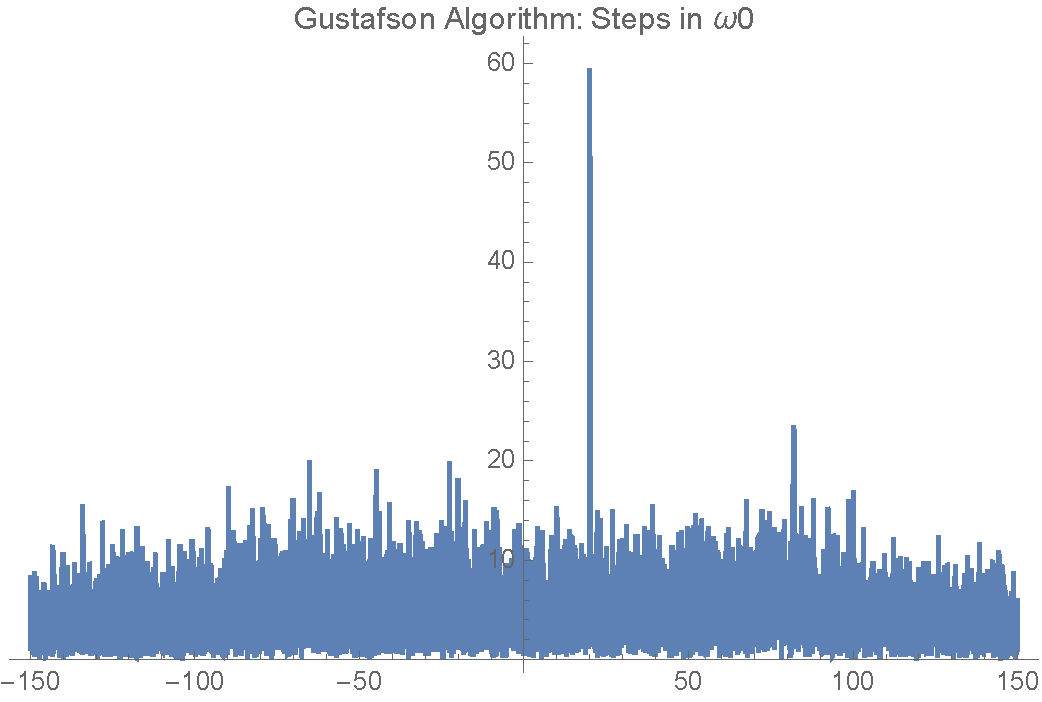
\includegraphics[width=.9\linewidth]{gustafsonAlgoStepInCarrier.pdf}
  		\caption{}
	\end{subfigure}%
	\begin{subfigure}{.5\textwidth}
  		\centering
  		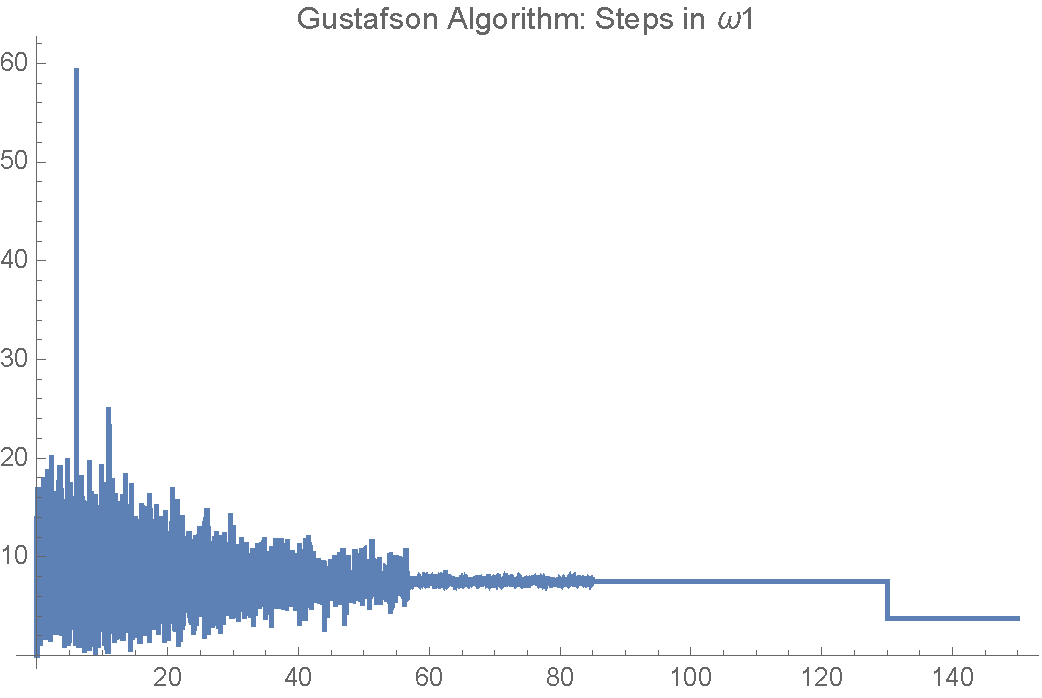
\includegraphics[width=.9\linewidth]{gustafsonAlgoStepInModFreq.pdf}
  		\caption{}
	\end{subfigure}
	\begin{subfigure}{.5\textwidth}
  		\centering
  		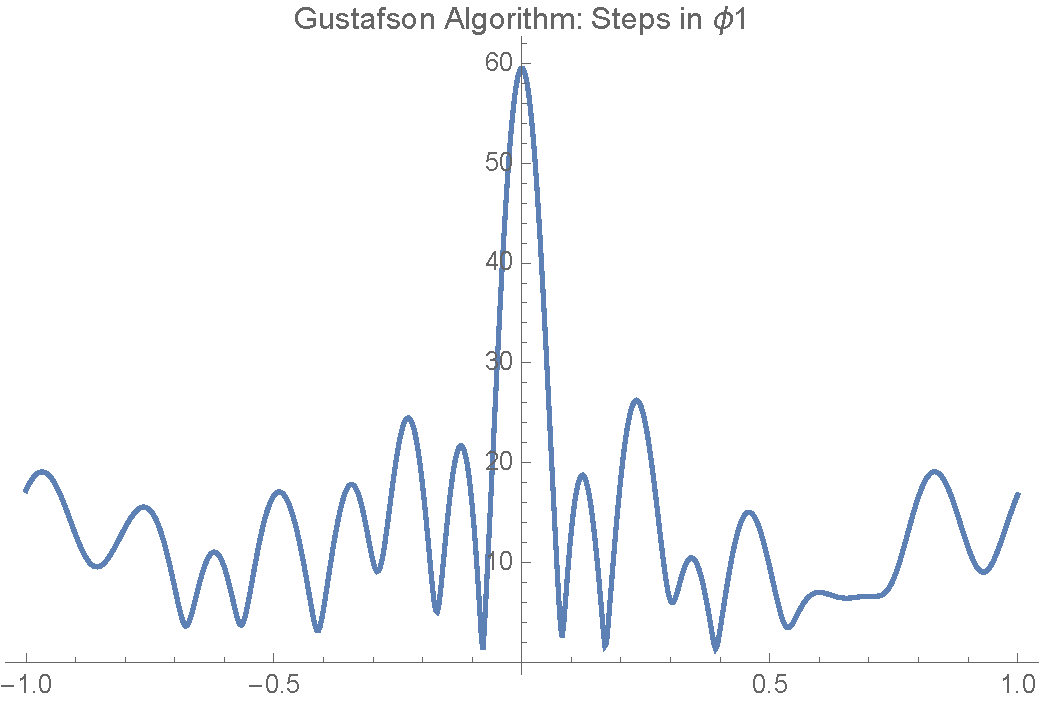
\includegraphics[width=.9\linewidth]{gustafsonAlgoStepInPhi1.pdf}
  		\caption{}
	\end{subfigure}%
	\begin{subfigure}{.5\textwidth}
  		\centering
  		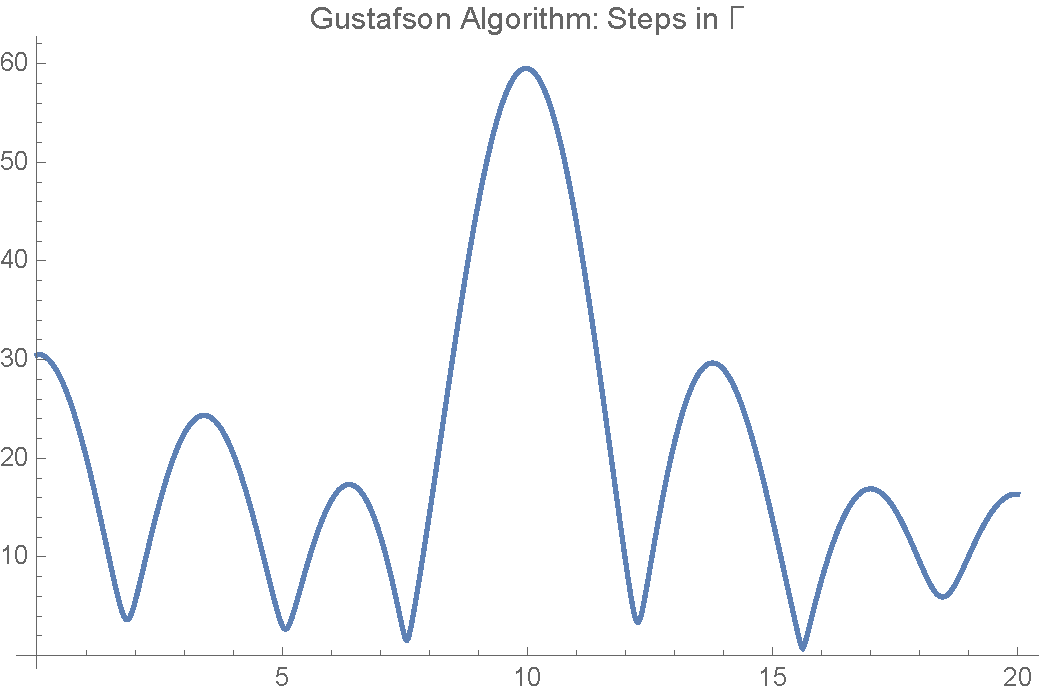
\includegraphics[width=.9\linewidth]{gustafsonAlgoStepInGamma.pdf}
  		\caption{}
	\end{subfigure}
	\caption{\label{fig:} Sampeling Rate = 300Hz, Carrier = 20Hz, Mod Frequency = 6Hz, Mod Index = 10, Time Series Duration = 10s}
\end{figure*}


\section{Conclusion}
Recap the benifits of working in the frequency domain vs the time domain.
It is the belief of this author that the methods outlined in this paper are unlikely to be useful for searching for gravitational waves.  


\appendix
\section{The Fourier Transform of The Complex Function}
The results this and the following section are quite surprising.  Looking at the instentanious frequency of a frequency modulated wave, it takes on every value between $\omega_0 \pm \omega_1$.  There are an uncountably infinite number of frequencies in this band, but essentially every frequency in this band does not appear in the Fourier Transform!  In fact, there are only two or three of these frequencies present in the Fourier Transform.  Moreover the bandwidth for a frequency modulated wave is infinite.  A countably infinite number of frequencies called \textit{sidebands} are evenly sapced at integer multiples of $\omega_1$ from the \textit{carrier frequency} $\omega_0$.  Interestingly for particular values of the \textit{modulation index} $\Gamma$ it is possible for the carrier frequency to not be present in the Fourier Transform!  This occures at the zeros of the zeroth Bessel Function.

%I BELIEVE I FORGOT SOME FACTORS OF 2PI HERE!!
\begin{align}
\mathcal{F}_t \left[ h_0 e^{i\left( \omega_0 t + \phi_0 + \Gamma \cos( \omega_1 t + \phi_1 ) \right)} \right]
&= h_0 e^{i\phi_0} \mathcal{F}_t \left[ e^{i\omega_0 t} e^{i\Gamma \cos(\omega_1 t + \phi_1)} \right]											\\
&= h_0 e^{i\phi_0} \mathcal{F}_t \left[ e^{i\omega_0 t} \right] \star \mathcal{F}_t \left[ e^{i\Gamma \cos(\omega_1 t + \phi_1)} \right]		\\
&= h_0 e^{i\phi_0} \delta(\omega - \omega_0) 
			\star \mathcal{F}_t \left[ \sum_{n=-\infty}^{\infty} e^{in\pi/2} J_n(\Gamma) e^{in(\omega_1 t + \phi_1)} \right]							\\
&= h_0 e^{i\phi_0} \delta(\omega - \omega_0) \star \sum_{n=-\infty}^{\infty} e^{in\pi/2} e^{in\phi_1} J_n(\Gamma) F_t \left[ e^{in\omega_1 t} \right]	\\
&= h_0 e^{i\phi_0} \delta(\omega - \omega_0) \star \sum_{n=-\infty}^{\infty} e^{in(\phi_1 + \pi/2)} J_n(\Gamma) \delta(\omega - n\omega_1)			\\
&= h_0 e^{i\phi_0} \sum_{n=-\infty}^{\infty} e^{in(\phi_1 + \pi/2)} J_n(\Gamma)  \delta(\omega - \omega_0) \star \delta(\omega - n\omega_1)			\\
&= h_0 e^{i\phi_0} \sum_{n=-\infty}^{\infty} e^{in(\phi_1 + \pi/2)} J_n(\Gamma)  \delta(\omega - \omega_0 - n\omega_1)
\end{align}

In this derivation we start by using the linearity of the Fourier Transform, then we invoke the Convolution Theorem, use the Jacobi-Anger Expansion, again use the linearity of the Fourier Transform, and the last few steps are simple Dirac Delta Function manipulations.

\section{The Fourier Transform of The Real-Valued Function}

\begin{align}
\mathcal{F}_t \left[ \Re \left\{ h_0 e^{i\left( \omega_0 t + \phi_0 + \Gamma \cos( \omega_1 t + \phi_1 ) \right)} \right\} \right]
&= \frac{1}{2} \mathcal{F}_t \left[ h_0 e^{i\left( \omega_0 t + \phi_0 + \Gamma \cos( \omega_1 t + \phi_1 ) \right)} 
                        + h_0 e^{-i\left( \omega_0 t + \phi_0 + \Gamma \cos( \omega_1 t + \phi_1 ) \right)} \right]			\\
&= \frac{h_0}{2} \left[ 
  e^{ i\phi_0} \mathcal{F}_t \left[ e^{i\left(  \omega_0 t + \Gamma \cos( \omega_1 t + \phi_1 ) \right)} \right] 
+ e^{-i\phi_0} \mathcal{F}_t \left[ e^{i\left( -\omega_0 t - \Gamma \cos( \omega_1 t + \phi_1 ) \right)} \right] 
\right]
\end{align}

From the previous section we see that

\begin{align}
\mathcal{F}_t \left[ e^{i(\omega_0 t + \Gamma \cos(\omega_1 t + \phi_1))} \right] 
= \sum_{n=-\infty}^{\infty} e^{in(\phi_1 + \pi/2)} J_n(\Gamma)  \delta(\omega - \omega_0 - n\omega_1)
\end{align}

and by replacing $\omega_0$ with $-\omega_0$ and $\Gamma$ with $-\Gamma$, and using the fact that $J_n(-\Gamma) = (-1)^n J_n (\Gamma)$ we also have

\begin{align}
\mathcal{F}_t \left[ e^{i(-\omega_0 t - \Gamma \cos(\omega_1 t + \phi_1))} \right] 
= \sum_{n=-\infty}^{\infty} e^{in(\phi_1 - \pi/2)} J_n(\Gamma)  \delta(\omega + \omega_0 - n\omega_1)
\end{align}

so the Fourier Transform of the real part of our frequency/phase modulated signal is

\begin{align}
\begin{split}
\mathcal{F}_t \left[ \Re \left\{ h_0 e^{i\left( \omega_0 t + \phi_0 + \Gamma \cos( \omega_1 t + \phi_1 ) \right)} \right\} \right]
= \frac{1}{2} h_0 \left[ e^{ i\phi_0} \sum_{n=-\infty}^{\infty} e^{in(\phi_1 + \pi/2)} J_n(\Gamma)  \delta(\omega - \omega_0 - n\omega_1) \right.	\\
+ \left. e^{-i\phi_0} \sum_{n=-\infty}^{\infty} e^{in(\phi_1 - \pi/2)} J_n(\Gamma)  \delta(\omega + \omega_0 - n\omega_1) \right]					\\
= \frac{1}{2} h_0 \sum_{n=-\infty}^{\infty} e^{in\phi_1} J_n (\Gamma) \left[ e^{i(\phi_0 + n\pi/2)} \delta(\omega - \omega_0 - n\omega_1) \right.	\\
+ \left. e^{-i(\phi_0 + n\pi/2)} \delta(\omega + \omega_0 - n\omega_1) \right]
\end{split}
\end{align}


%\begin{align}
%\label{eqn:realFourierTransform}
%\Aboxed{\frac{1}{2} h_0 \sum_{n=-\infty}^{\infty} e^{in\phi_1} J_n (\Gamma) \left[ e^{i(\phi_0 + n\pi/2)} \delta(\omega - \omega_0 - n\omega_1)
%+ e^{-i(\phi_0 + n\pi/2)} \delta(\omega + \omega_0 - n\omega_1) \right]}
%\end{align}

\begin{align}
\label{eqn:realFourierTransform}
\hat{f}(\omega) = 
\frac{1}{2} h_0 \sum_{n=-\infty}^{\infty} e^{in\phi_1} J_n (\Gamma) \left[ e^{i(\phi_0 + n\pi/2)} \delta(\omega - \omega_0 - n\omega_1)
+ e^{-i(\phi_0 + n\pi/2)} \delta(\omega + \omega_0 - n\omega_1) \right]
\end{align}

Notice that, by taking the fourier transform of just the real part of our frequency modulated function it has added the terms in red.  (Go into more detail why that is)  The other important change is that the $X_n$ and $Y_n$ terms were added (Again, go into more detail why that is).

\pagebreak

\section{Selected Waveforms}


\begin{figure}[H]
	\centering
	\begin{subfigure}{.5\textwidth}
  		\centering
  		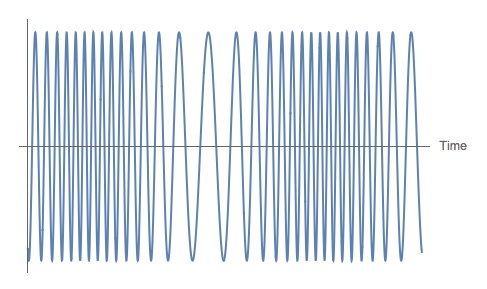
\includegraphics[width=.9\linewidth]{classicSignal.png}
  		\caption{When the carrier frequency is much higher than the modulation frequency the frequency modulated wave is "nice". $\Gamma = 9.88, \omega_0 = 3.62, \omega_1 = 0.21, \phi_1 = 3.14$ \label{fig:niceSignal}}
	\end{subfigure}%
	\begin{subfigure}{.5\textwidth}
  		\centering
  		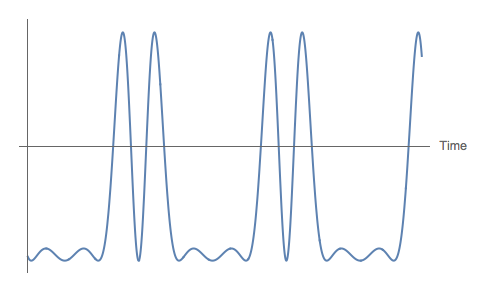
\includegraphics[width=.9\linewidth]{interestingSignal.png}
  		\caption{When the carrier frequency is a multiple of the modulation frequency one can get exotic waveforms.  One example of the exotic signals cyclic frequency modulation can produce.  $\Gamma = 2.88, \omega_0 = 1.5, \omega_1 = 0.75, \phi_1 = 0$ \label{fig:interestingSignal}}
	\end{subfigure}
	\begin{subfigure}{.5\textwidth}
  		\centering
  		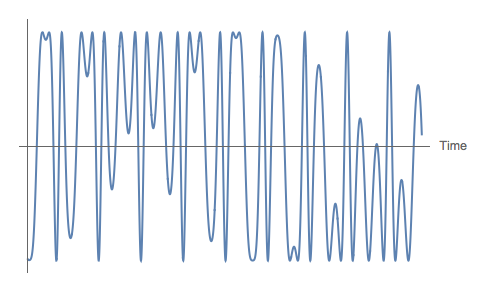
\includegraphics[width=.9\linewidth]{nastySignal.png}
  		\caption{When the carrier and modulation frequencies are almost equal the resulting FM wave is not so nice.  This is a particularly nasty waveform that could be mistaken as noise by looking at it. $\Gamma = 3, \omega_0 = 0.42, \omega_1 = 0.46, \phi_1 = 0.1$ \label{fig:nastySignal}}
	\end{subfigure}
\end{figure}

% --------------------------- Code for the bibliography ---------------------------------------------------------------------------------
\bibliography{shgBibliographyCopy}



\end{document}